\documentclass[12pt,a4paper]{article}
\usepackage[top=2.7cm, bottom=2cm, left=2cm, right=2cm]{geometry}
\usepackage[utf8]{inputenc}
\usepackage{CJKutf8}
\usepackage{enumitem}
\usepackage{verbatim}
\usepackage[normalem]{ulem}


%% Useful packages
\usepackage{amsmath,amssymb}
% \usepackage{subfigure}
\usepackage{graphicx,wrapfig}
\usepackage[dvipsnames,table]{xcolor}
\usepackage[table]{xcolor}
\usepackage{url}
\usepackage{setspace}
\usepackage[colorlinks=true,anchorcolor=black,linkcolor=Blue,urlcolor=RoyalBlue]{hyperref}
\usepackage[linesnumbered,ruled,vlined]{algorithm2e}
\usepackage{threeparttable}
\usepackage{arydshln}
\usepackage{tikz}
\usepackage{blindtext}
\usepackage{titlesec}
\usepackage{courier}
\usepackage{pdfpages}

\usepackage{lastpage}
\usepackage{fancyhdr}
\usepackage{makecell}

\setlength{\headheight}{0pt}
\renewcommand{\headrulewidth}{1pt} % remove lines
\renewcommand{\footrulewidth}{0pt}
\pagestyle{fancyplain}
\fancyhf{}


\newcommand{\hynote}[1]{{\bf\footnotesize \color{red}[YPH: #1]}}

\lhead{
  \textcolor{Gray}{Group 2}
}
\rhead{
  \begin{CJK}{UTF8}{bkai}
  \textcolor{Gray}{實驗結報}
  \end{CJK}
}
\lfoot{
   \textcolor{Gray}{May 13}
  }
\rfoot{
  \thepage/\pageref{LastPage}
  }

\title{\vspace{-0.5cm}
       {\bf \textcolor{black}{{\LARGE 
       \begin{CJK}{UTF8}{bkai}
       實驗物理學(二)\\
       \vspace{6pt}
        實驗報告\\
       % \vspace{60pt}
       % Fundamental Python\\
       % \vspace{6pt}
       % Basic Usage of Python
       \end{CJK}
       }}
       }
       }
\author{}
\date{}

\begin{document}
\begin{CJK}{UTF8}{bkai}

\maketitle
\thispagestyle{empty}

\vspace{10cm}
\begin{center}
{\bf \LARGE \vspace{-11cm} Fundamental Python\\
\vspace{0.25cm} Chi-square fitting - 3}\\
\vspace{13cm}
{\large Group 2}\\ \vspace{12pt}
{\large \makebox[3em][s]{洪\hspace{\fill}瑜} B125090009}\\ \vspace{6pt}
{\large \makebox[3em][s]{黃巧涵}  B122030003}\\ \vspace{6pt}
{\large \makebox[3em][s]{洪懌平} B102030019}\\ \vspace{12pt}
{\large 2025/05/13}\\
\end{center}



\clearpage
%--------------------------------------------------------------%
\vspace{2cm}
\begin{center}
{\large\bf\sc 摘要}
\end{center}

\noindent

本次實驗著重於了解卡方擬合(Chi-square fitting)與統計檢定中 p-value 的應用與意義。透過兩個練習(Practice 1 與 Practice 2),我們分別以自行設定的二次函數產生含隨機誤差的模擬數據,進行擬合分析,計算對應的卡方值與 p-value,並探討其與模型合理性的關係。我們自行撰寫 p-value 計算器,並比較實驗所得的 p-value 分布與理論預測。進一步,我們利用顯著水準(significance level)判斷擬合是否合理,並對 p-value 與模型參數準確性之關聯進行實證討論。結果顯示,p-value 雖可反映擬合結果是否顯著偏離理論模型,但不應作為評估參數準確性的唯一指標。本實驗強調統計方法與視覺化工具在模型擬合與驗證中的重要性,對於日後進行更複雜的資料分析與科學建模具有實質助益。

\section{前言}
\hfill

在本周的課程內容,我們會從practice 1練習到p-value的意義和計算,以及其和$\chi^2$的關係;而在practice 2,則會著重在利用p-value去探討其與擬合結果好壞的關聯,並認識甚麼是significance level。

\subsection{P-value}
\hfill

在了解$P-value$前,需要先知道一些先備知識。
\begin{itemize}
    \item 虛無假設(null hypothesis)$H_0$:對某件事情預設為某種結果或狀態。
    \item 對立假說(alternative hypothesis)$H_1$:為虛無假設的對立面。
\end{itemize}

%\renewcommand{\arraystretch}{1.5}
\begin{table}[h]
    \centering
    \begin{tabular}{|c|c|c|}
        \hline
        &$H_0$為真&$H_1$為真($H_0$錯誤)\\
        \hline
        拒絕$H_0$&\makecell{錯誤判斷(第I型錯誤)\\發生機率$=\alpha$}&\makecell{正確判斷\\發生機率$= 1-\beta$} \\
        \hline
        接受$H_0$&\makecell{正確判斷\\發生機率$=1-\alpha$}&\makecell{錯誤判斷(第II型錯誤)\\發生機率$=\beta$}\\
        \hline
    \end{tabular}
    \caption{假設檢定中的判斷與錯誤類型}
    \label{tab:1}
\end{table}


接著來介紹甚麼是p-value,並且要怎麼透過觀察這個數值來判斷擬合的結果是否合理。

\begin{itemize}
    \item \textbf{p-value之定義}:在虛無假設的情況下,發生此統計結果、或更極端的結果之機率;所以p-value越小表示$H_0$為真時越不可能發生,即可推論$H_0$假設錯誤。
    \begin{enumerate}
        \item P-value的P是Probability的P,也就是描述事件發生的可能性。
        \item 計算p-value的前提是虛無假設為真。
    \end{enumerate}
\end{itemize}

\clearpage

我們使用$desmos$繪圖作為範例,用圖像化的方式更清楚的解釋$p-value$:
\begin{figure}[h]
    \centering
    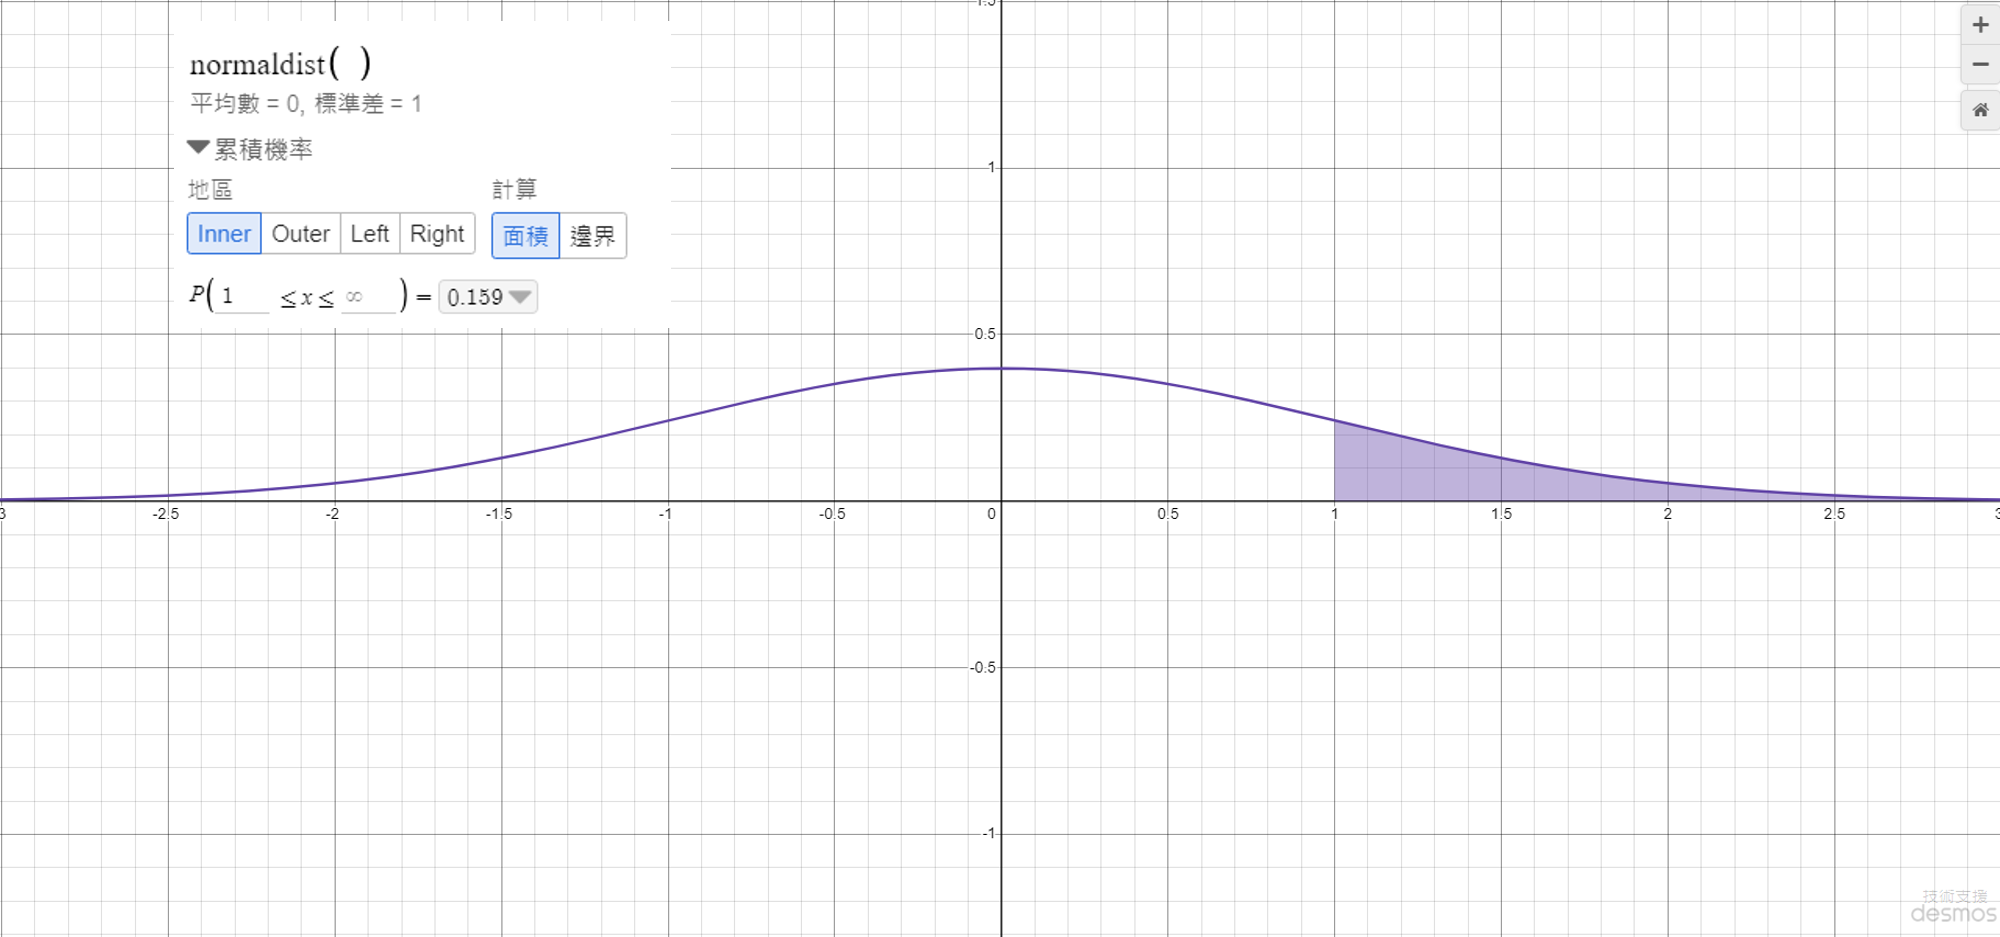
\includegraphics[width=0.8\linewidth]{figures/RF/desmos.png}
    \caption{利用常態分佈解釋p-value}
    \label{fig:desmos_1}
\end{figure}


Fig.\ref{fig:desmos_1}為一平均$\mu=0$、標準差$\sigma=1$之常態分佈的圖形,我們標示出在$1\le x\le \infty$這個範圍下,常態分佈下的面積,而其代表的意義是「觀察值大於等於1的機率」,在圖的左上角,可看見$P=0.159$,說明在虛無假設成立的情況下,發生此事件的機率為$0.159$。

\begin{itemize}
    \item \textbf{p-value與$\chi^2$的關係}
\end{itemize}

在這裡,一樣使用$desmos$圖像化解釋:
\begin{figure}[h]
    \centering
    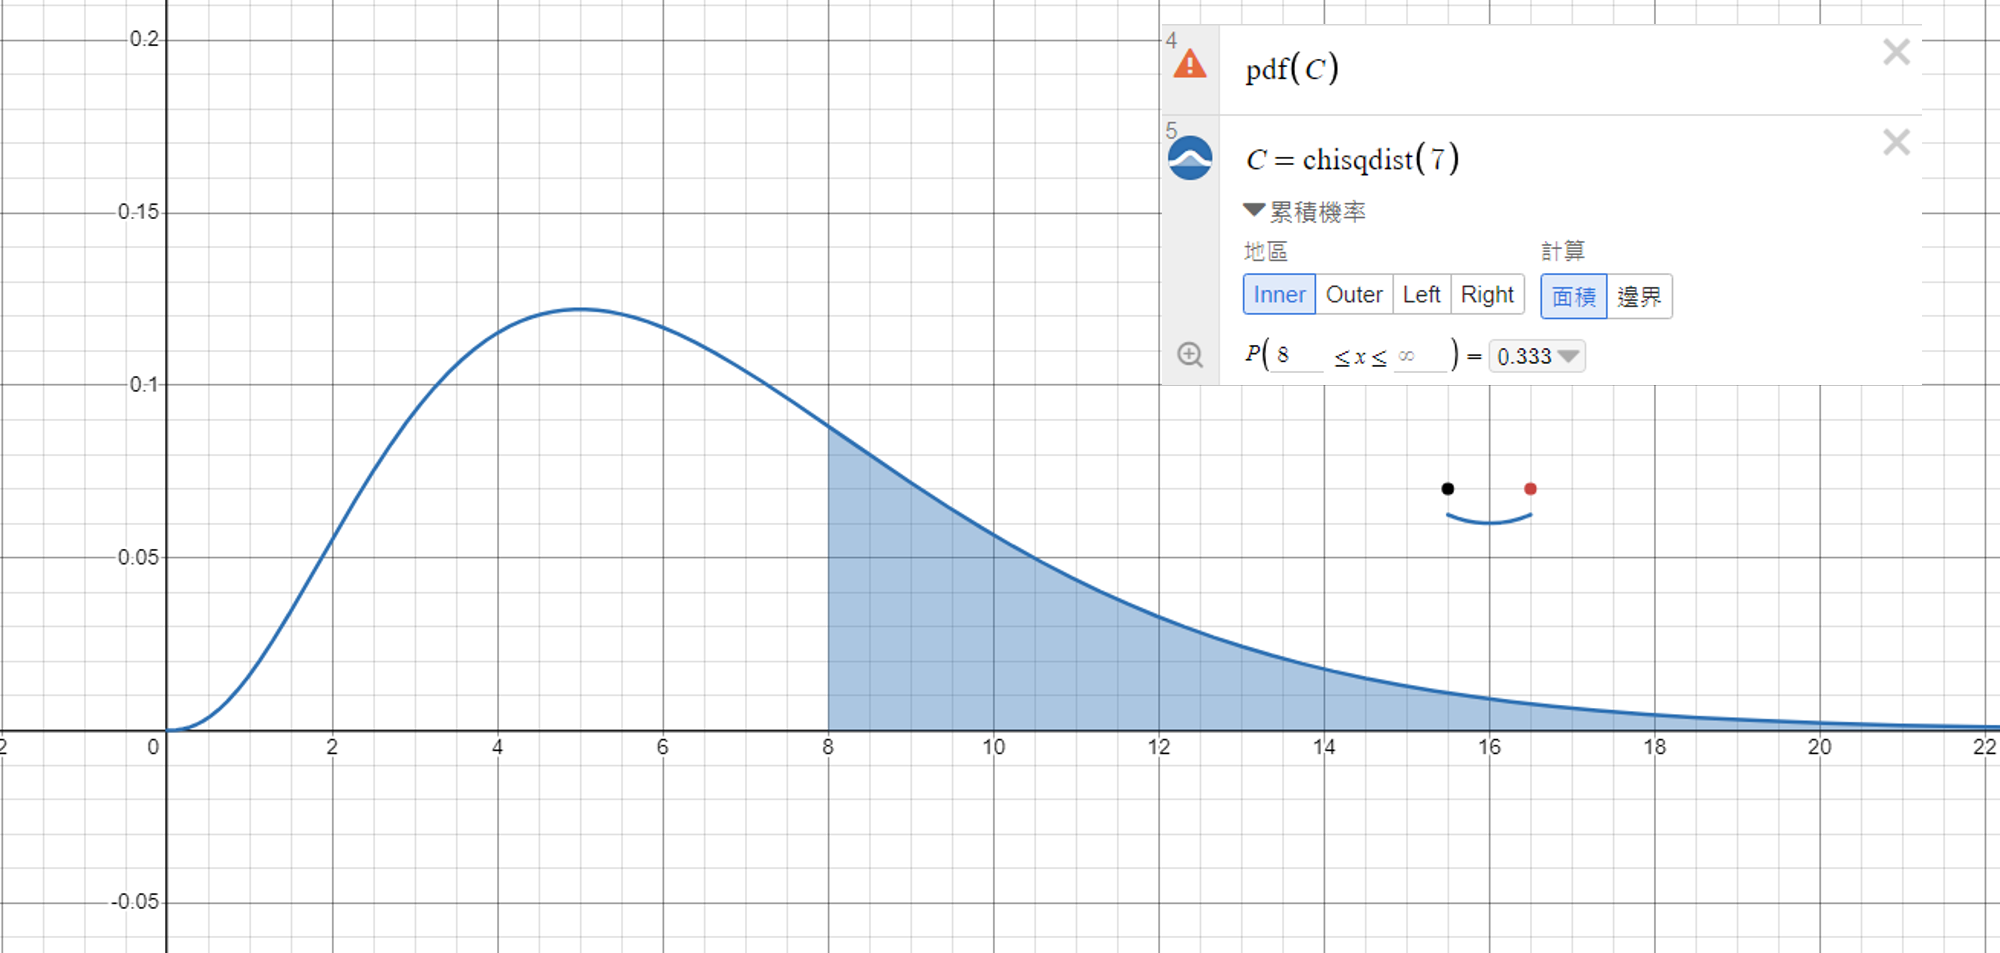
\includegraphics[width=0.8\linewidth]{figures/RF/desmos_3.png}
    \caption{利用PDF($dof=7$)解釋p-value與$\chi^2$的關係}
    \label{fig:desmos_2}
\end{figure}

Fig.\ref{fig:desmos_2}模擬一個$dof=7$時的PDF,而x軸為$\chi^2$值。假設我們實驗所得之$\chi^2=8$,那發生此事件的機率即為$8\le\chi^2$這個區間在PDF下的面積(也就是圖上所標示的藍色區塊),而這個機率就是p-value(假設$H_0$為真),由圖的右上角可知:$p-value=0.333$。\\

note: p-value不是$H_0$為真的機率,而是「$H_0$為真的前提下」,發生目前的統計結果或更極端的情況之機率。

\clearpage

\subsection{significance level}
\hfill

significance level是拒絕$H_0$、但其實$H_0$為真的機率;即為Tab.\ref{tab:1}上寫的「第I型錯誤」,發生機率為$\alpha$。可以把significance level想像成p-value的門檻,如果$p<\alpha$就拒絕$H_0$(放在本實驗的情況就是不接受這個擬合結果)。另一個相關的參數是信賴水準$\gamma=1-\alpha$,指的是我們對$H_0$為真時,建立的統計模型有多大的信心,例如假設現在信賴水準是95\%,表示如果重複做很多次實驗,有95\%的機率算出來的$\chi^2$會落在此範圍內;從另一個角度來看就是有5\%的機率我們會拒絕這個虛無假設,所以p-value會小於$0.05$。

在本次的實驗中,我們設定significance level為上下各5\%;分別排除欠擬合($\chi^2$過大)與過擬合($\chi^2$過小)這兩種情況,因此得到的$\chi^2$要落在這兩個區間內,這個模型才是可被接受的。

\begin{figure}[h]
    \centering
    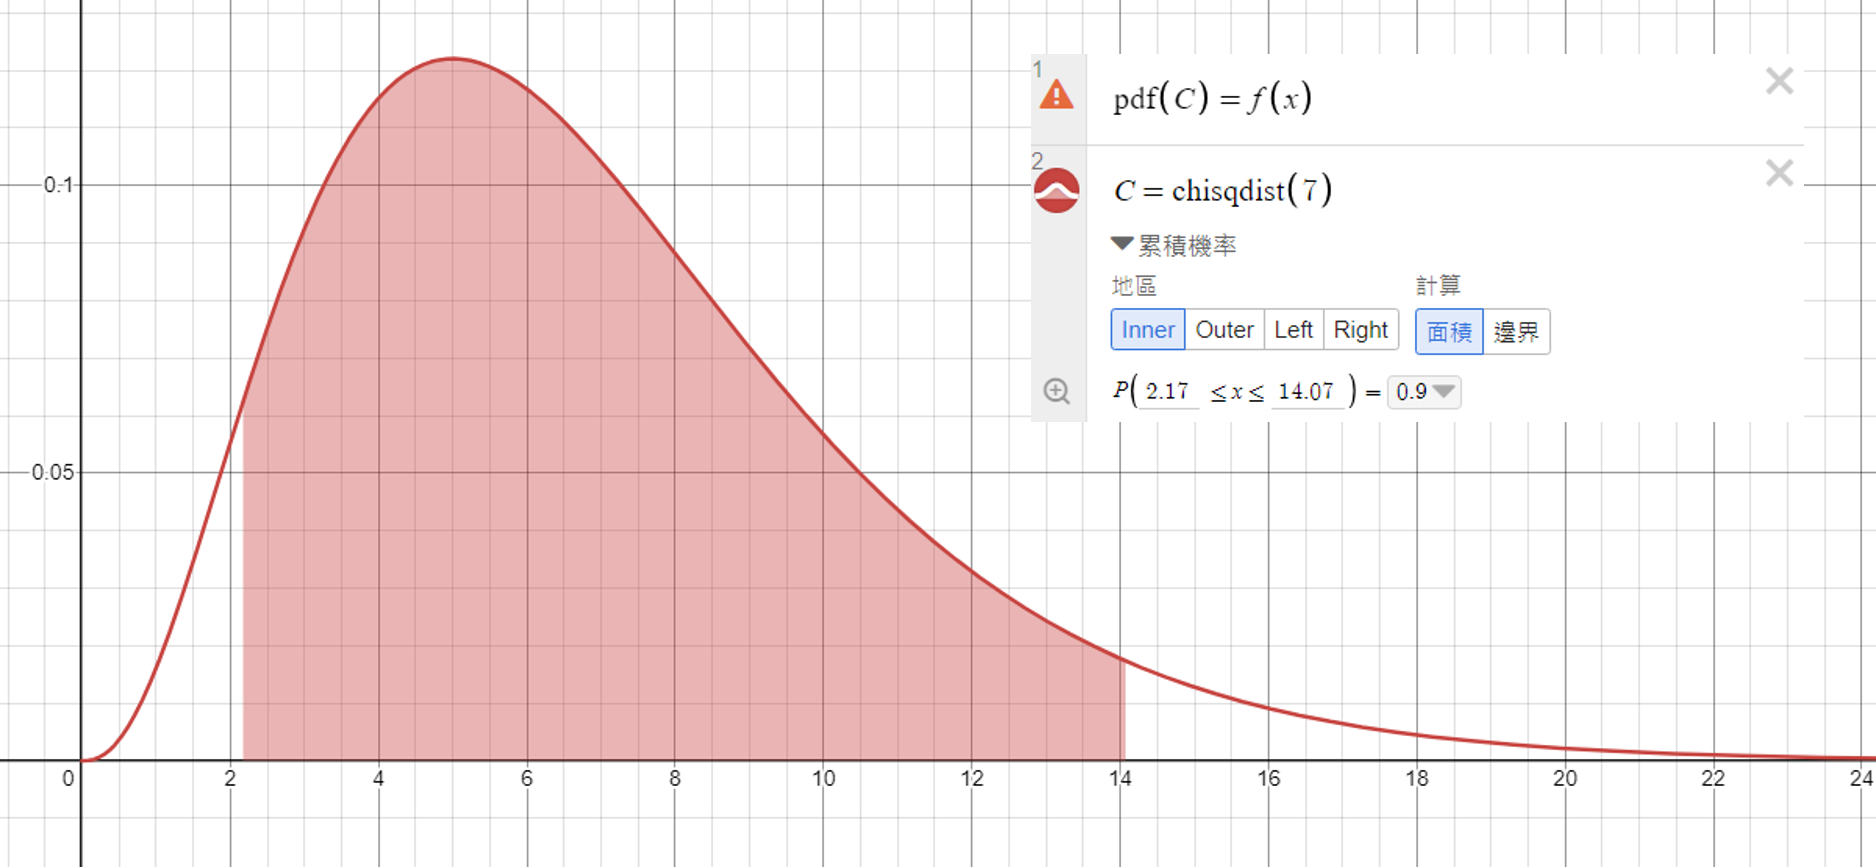
\includegraphics[width=1\linewidth]{figures/RF/desmos_4.png}
    \caption{紅色面積標示出$5\%<p-value<95\%$的範圍,實驗所得之$\chi^2$需落在此範圍方可接受}
    \label{fig:sig_level}
\end{figure}





%%%%%%%%%%%%%%%%%%%%%%%%%%%%%%%%5
\clearpage
\section{實驗步驟}

\subsection{Practice 1}
\hfill

\begin{enumerate}
    \item By using previous knowledge, choose your own function to generate data points.
    \begin{figure}[h]
        \centering
        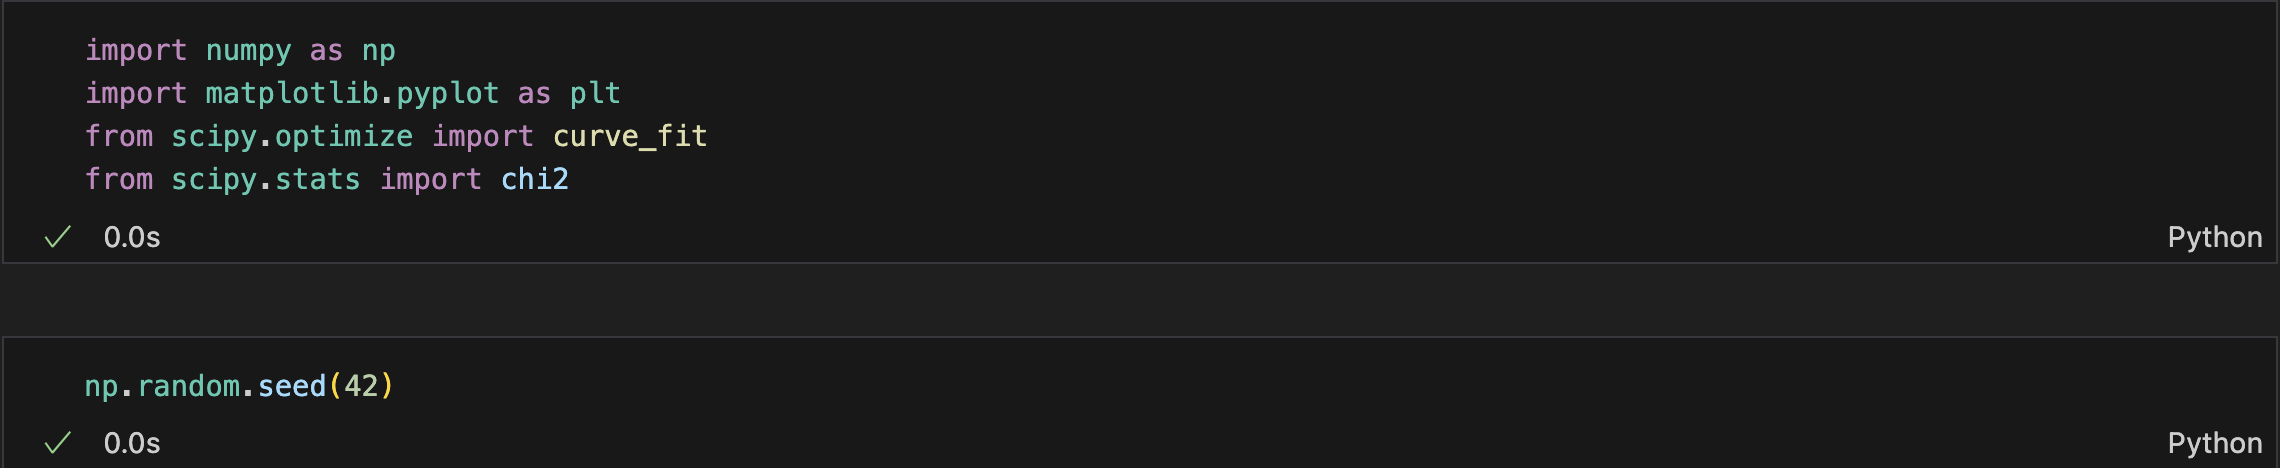
\includegraphics[width=1\linewidth]{figures/code/practice_1/code_1_1.png}
        % \caption{Caption}
        \label{fig:code_1_1}
    \end{figure}
    \item Generate 1000 sets of data points with the same function with normally distributed random noise.
    \begin{figure}[h]
        \centering
        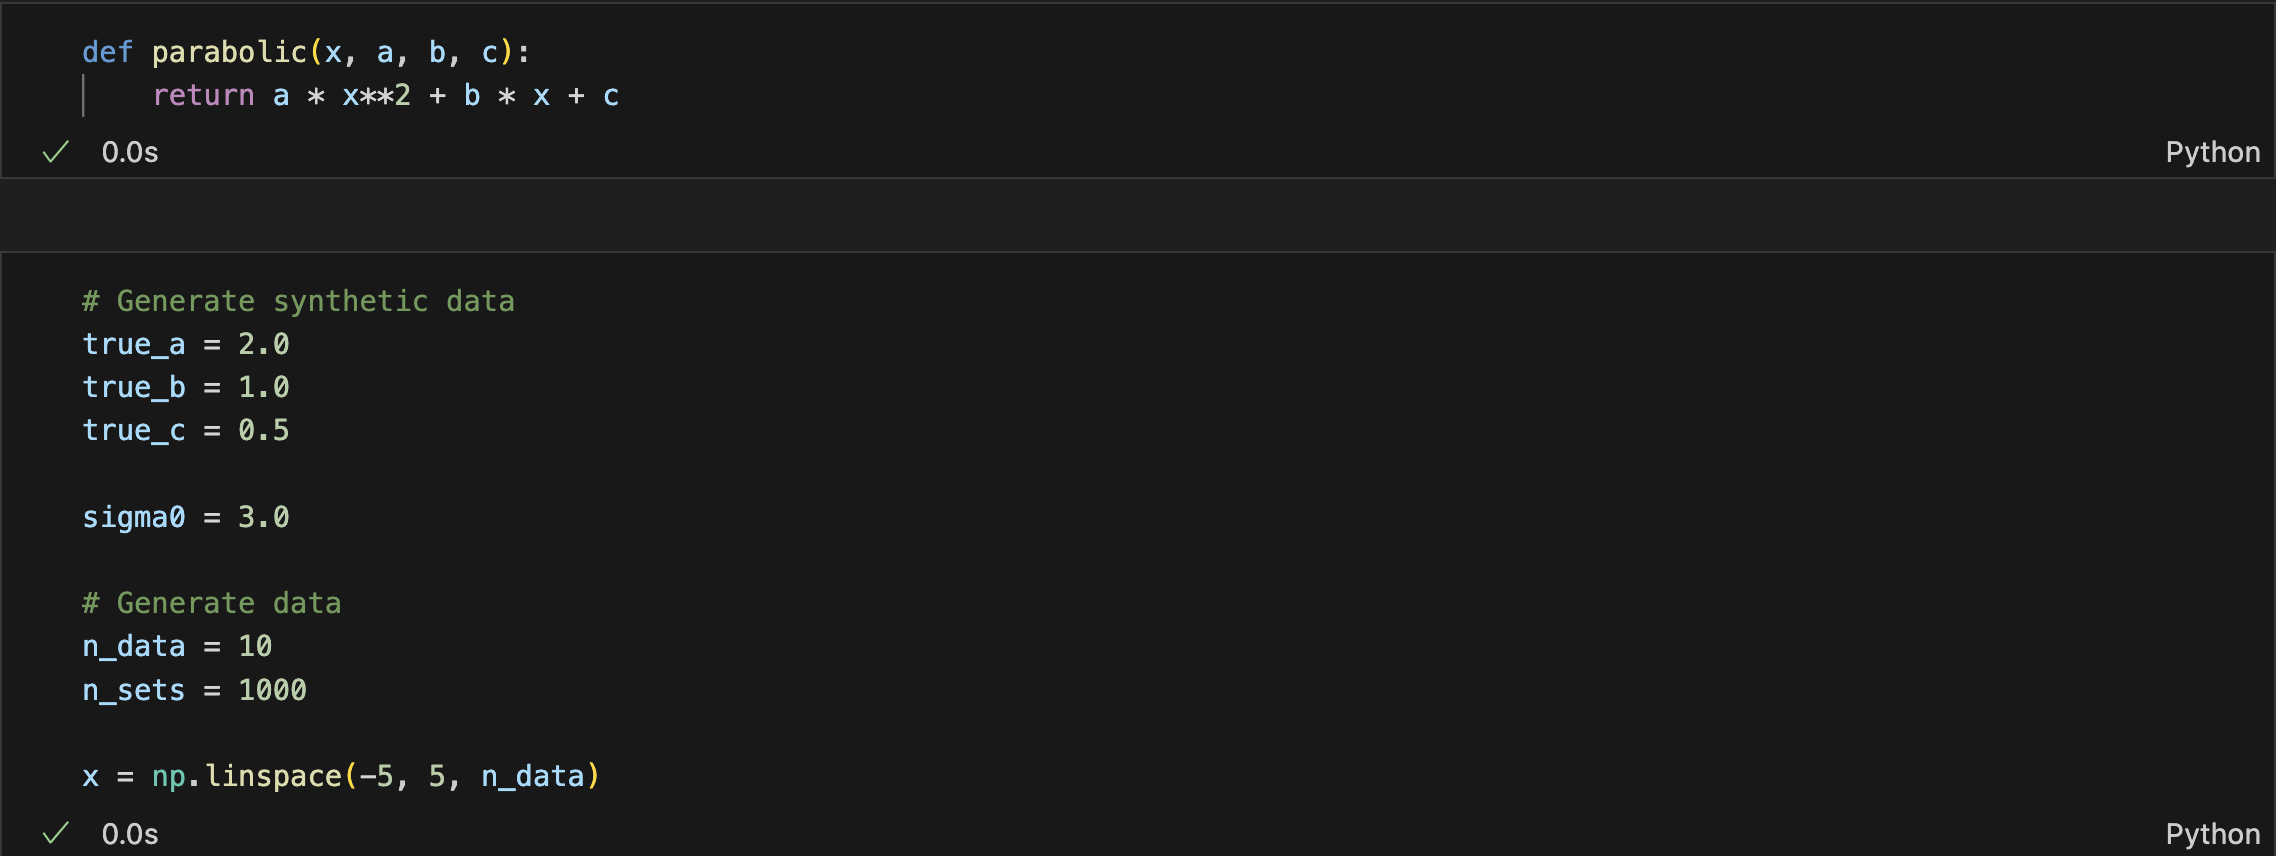
\includegraphics[width=1\linewidth]{figures/code/practice_1/code_1_2.png}
        % \caption{Caption}
        \label{fig:code_1_2}
    \end{figure}
    \clearpage
    \item Fit these data points with the function you used to generate the data points.
    \item Calculate the $\chi^2$ values of each fitting result.
    \begin{figure}[h]
        \centering
        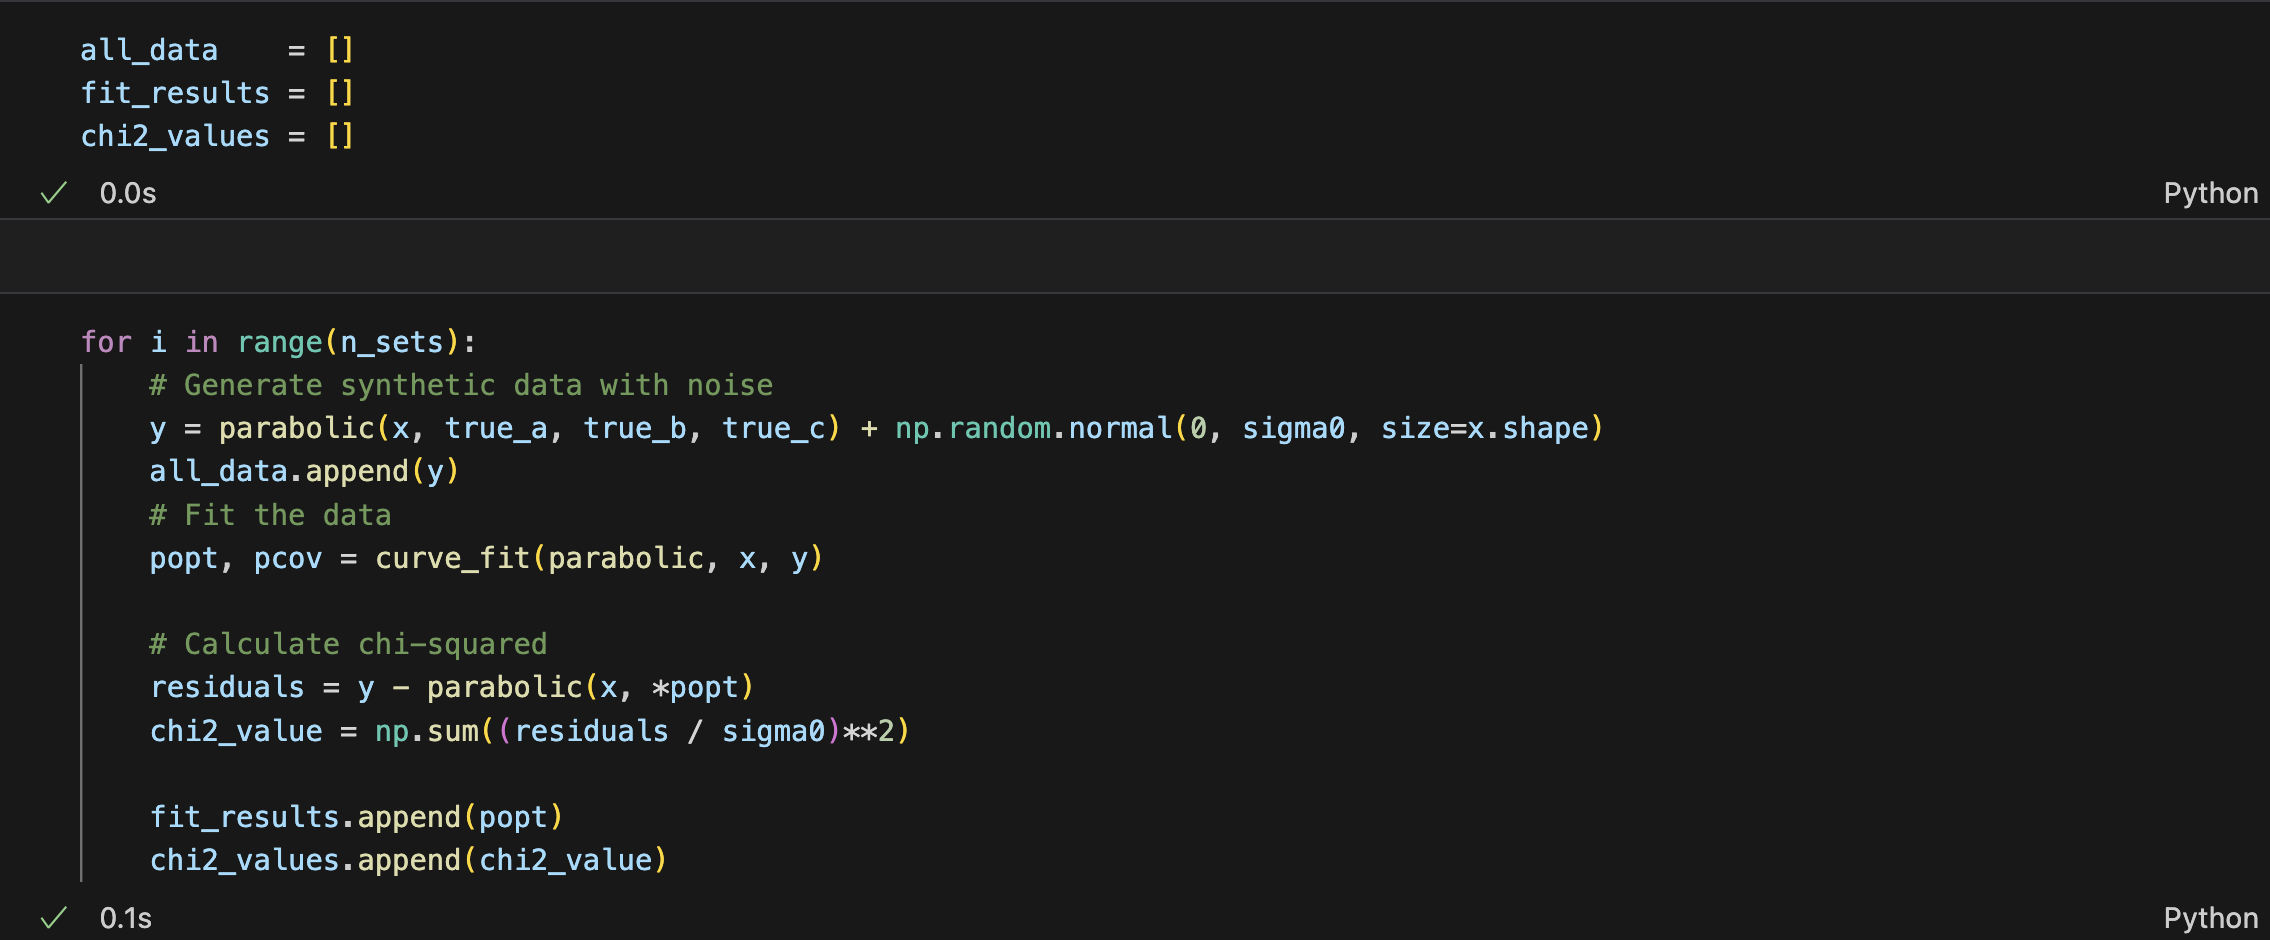
\includegraphics[width=1\linewidth]{figures/code/practice_1/code_1_3.png}
        % \caption{Caption}
        \label{fig:code_1_3}
    \end{figure}
    % \item Explain how to calculate the \textbf{p-value}.
    \item Create your own \textbf{p-value} calculator to calculate the \textbf{p-value} of each $\chi^2$ instead of using functions in \texttt{scipy.stats}.
    \begin{figure}[h]
        \centering
        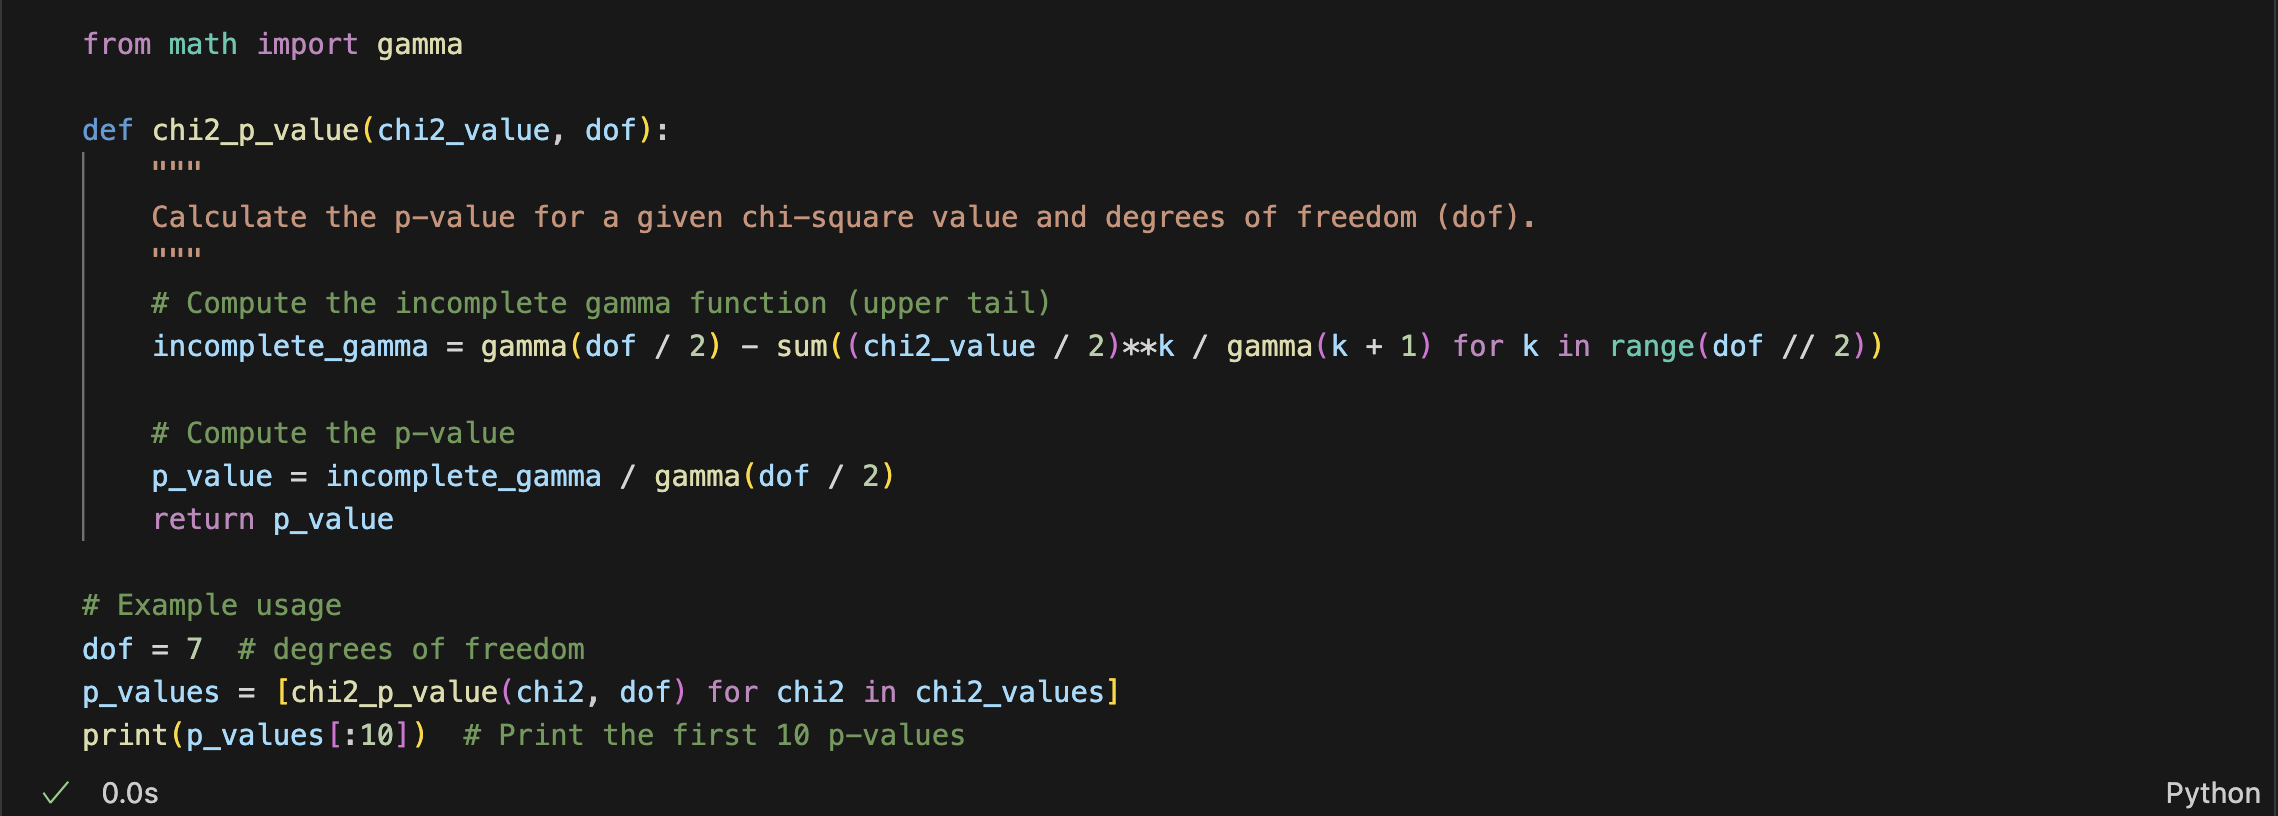
\includegraphics[width=1\linewidth]{figures/code/practice_1/code_1_6.png}
        % \caption{Caption}
        \label{fig:code_1_6}
    \end{figure}
    \begin{figure}[h]
        \centering
        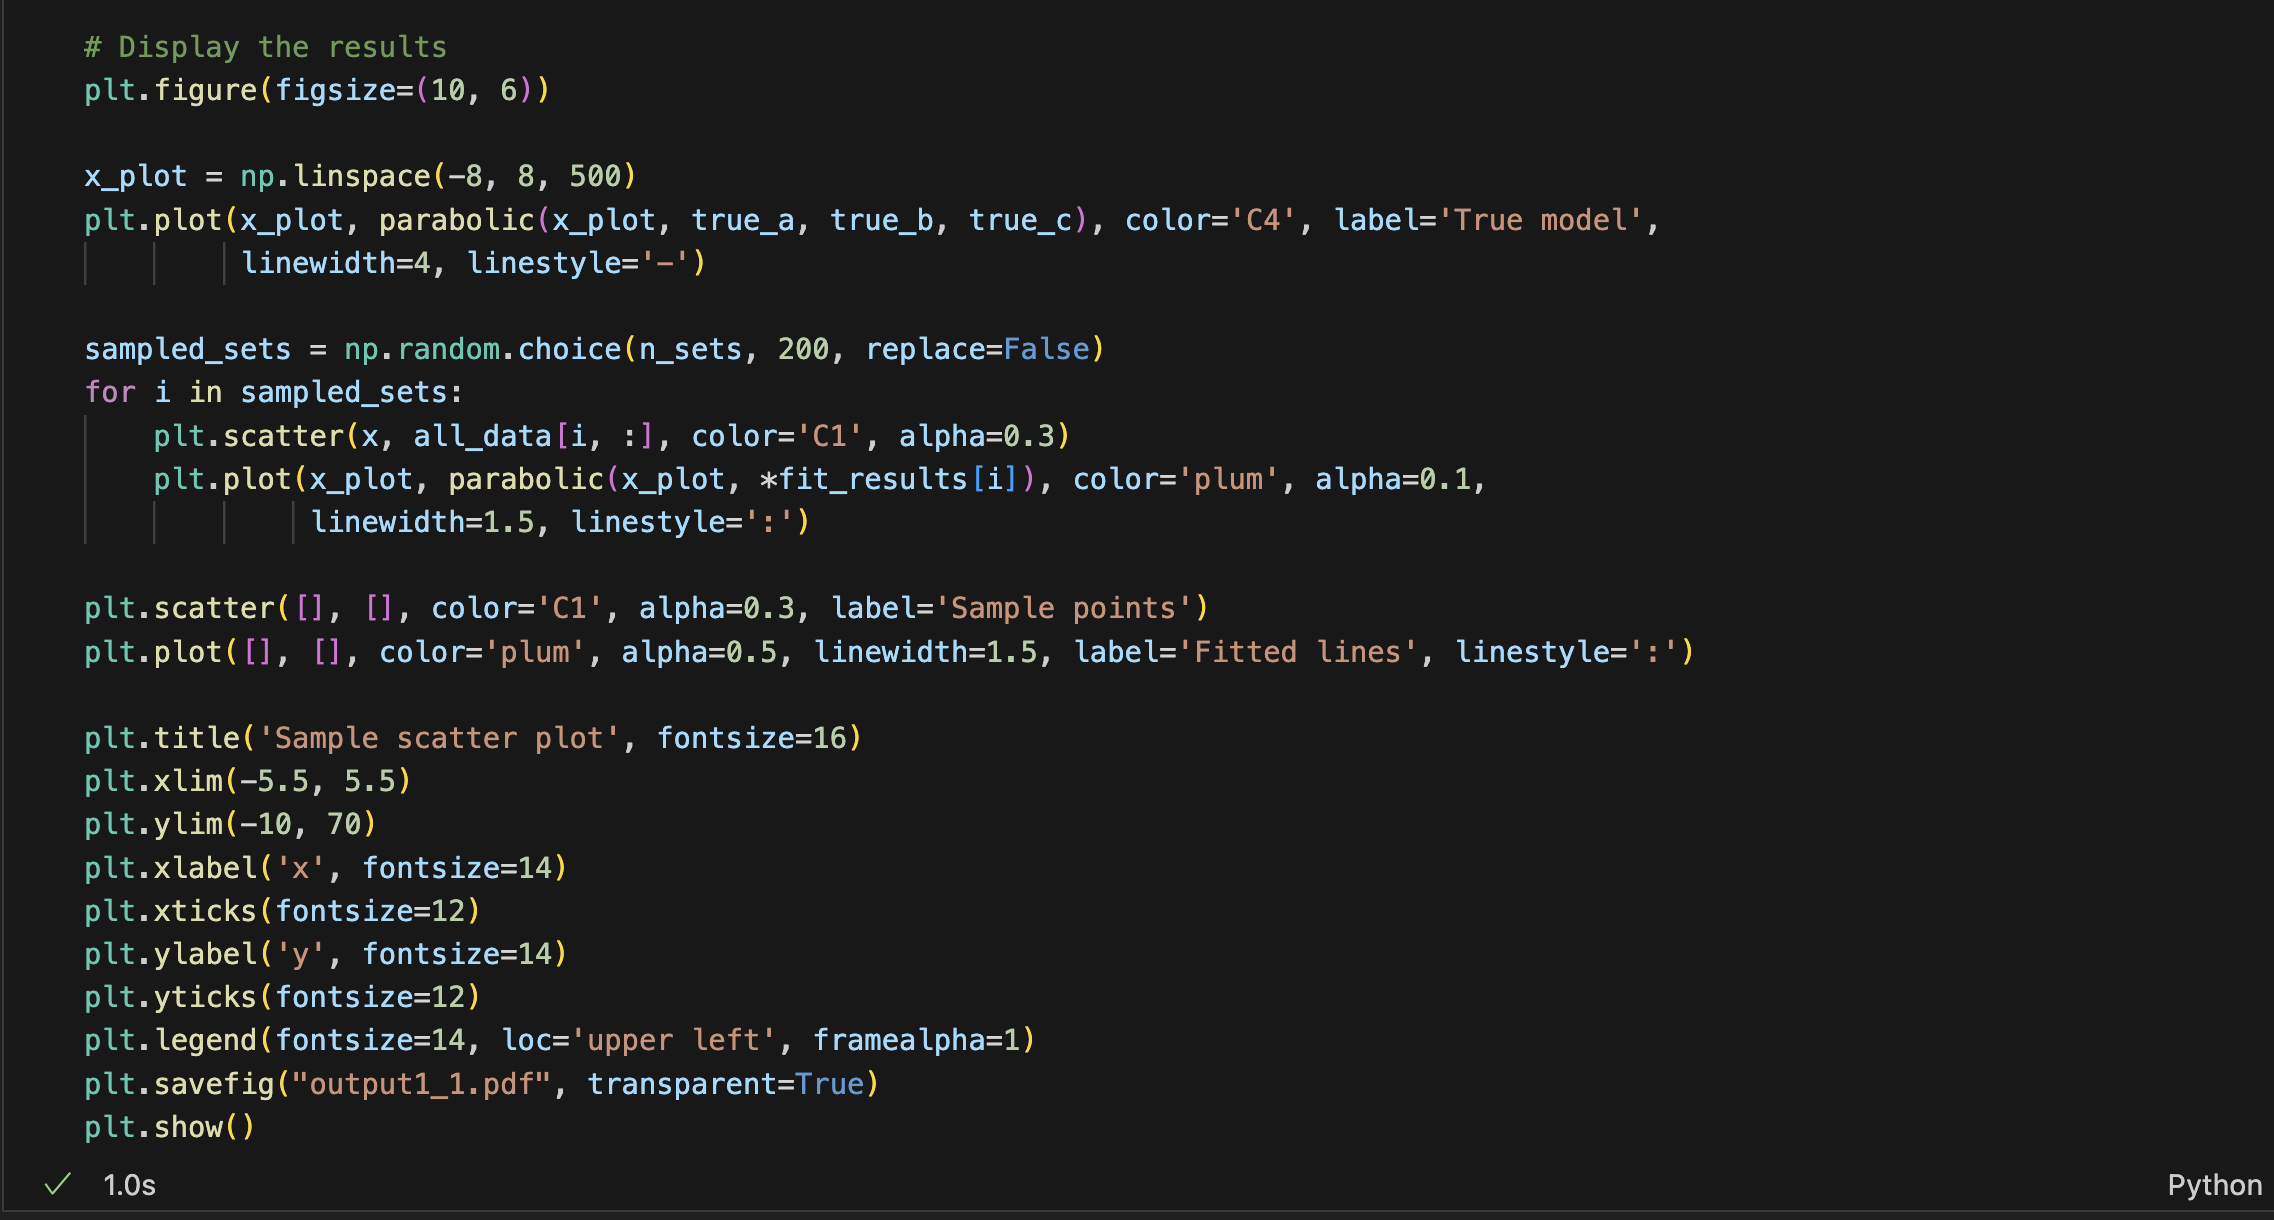
\includegraphics[width=1\linewidth]{figures/code/practice_1/code_1_4.png}
        % \caption{Caption}
        \label{fig:code_1_4}
    \end{figure}
    % \clearpage
    \item Plot the histogram of $\chi^2$.
    \begin{figure}[h]
        \centering
        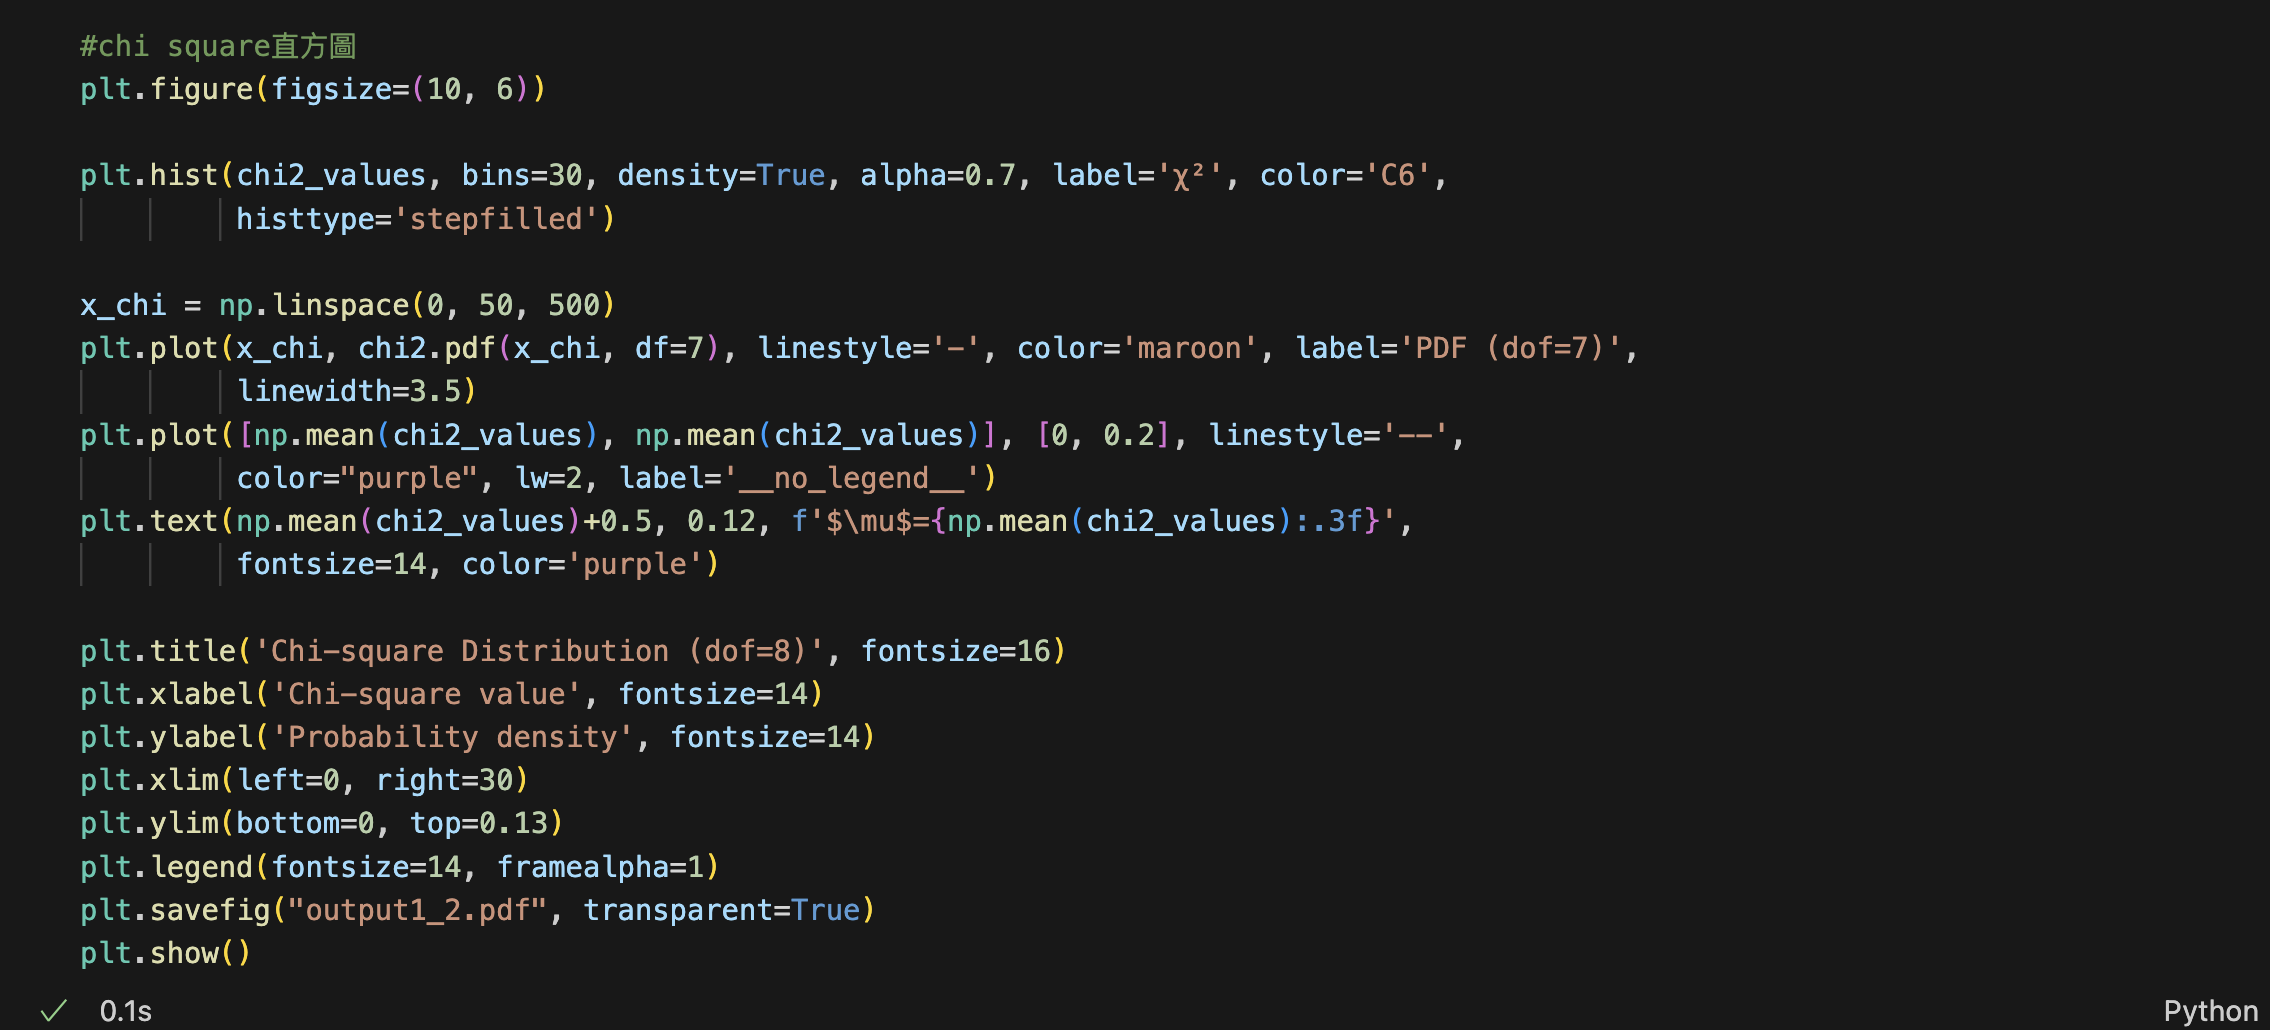
\includegraphics[width=1\linewidth]{figures/code/practice_1/code_1_5.png}
        % \caption{Caption}
        \label{fig:code_1_5}
    \end{figure}
    \clearpage
    \item Mark a certain $\chi^2$ value with its corresponding \textbf{p-value} on the histogram.
    \begin{figure}[h]
        \centering
        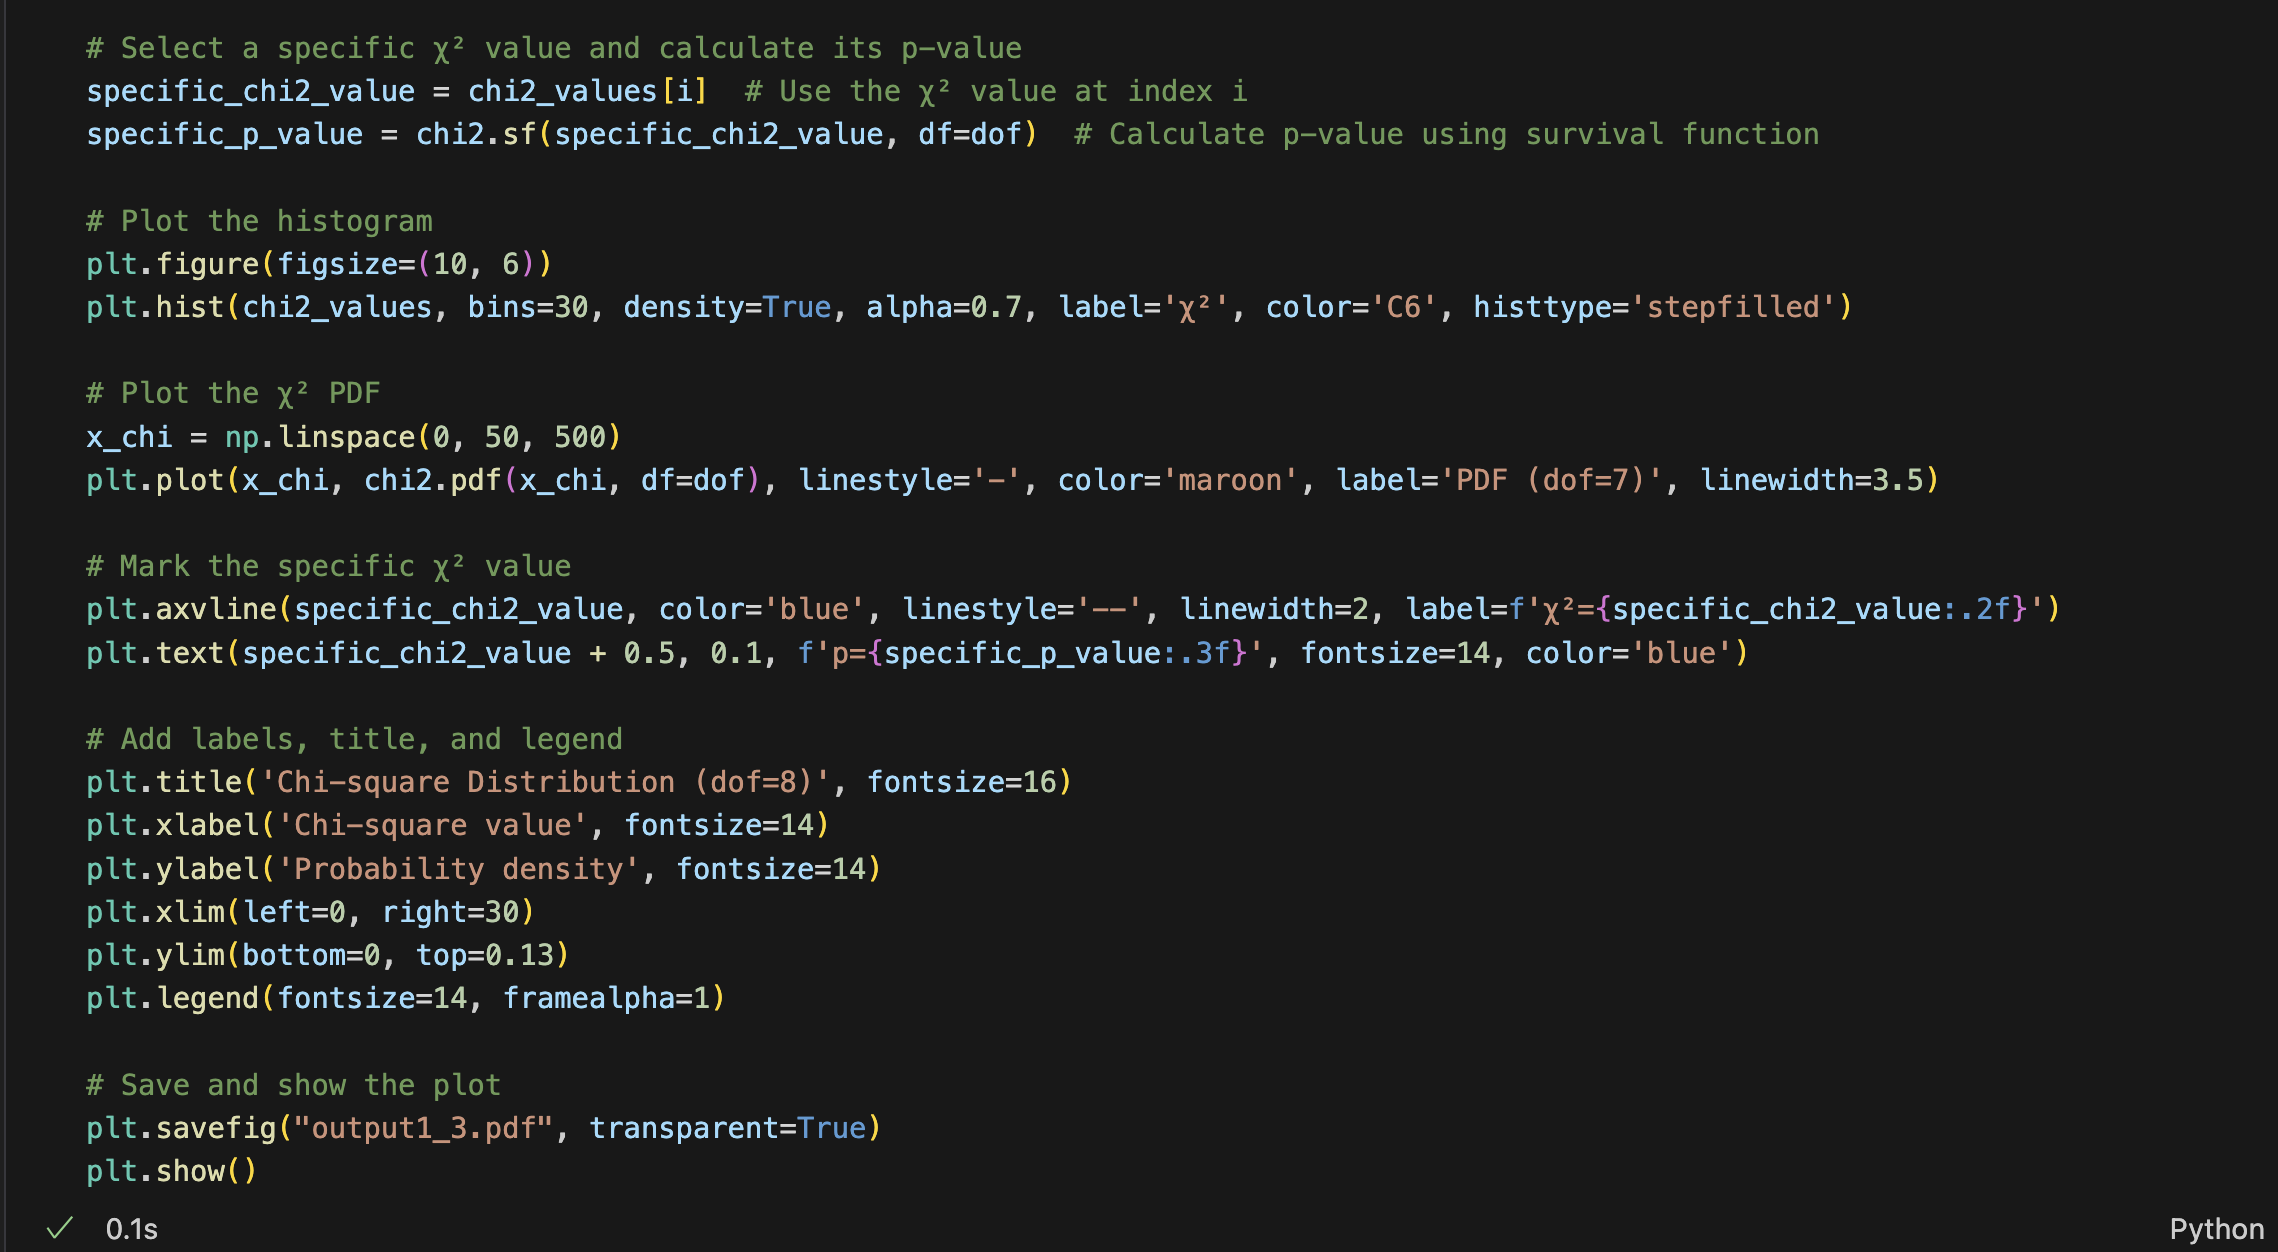
\includegraphics[width=1\linewidth]{figures/code/practice_1/code_1_7.png}
        % \caption{Caption}
        \label{fig:code_1_7}
    \end{figure}
\end{enumerate}

% \clearpage
\subsection{Practice 2}
\hfill

\begin{enumerate}
    \item Using prior knowledge, select an appropriate function with noise to generate your dataset.
    \begin{figure}[h]
        \centering
        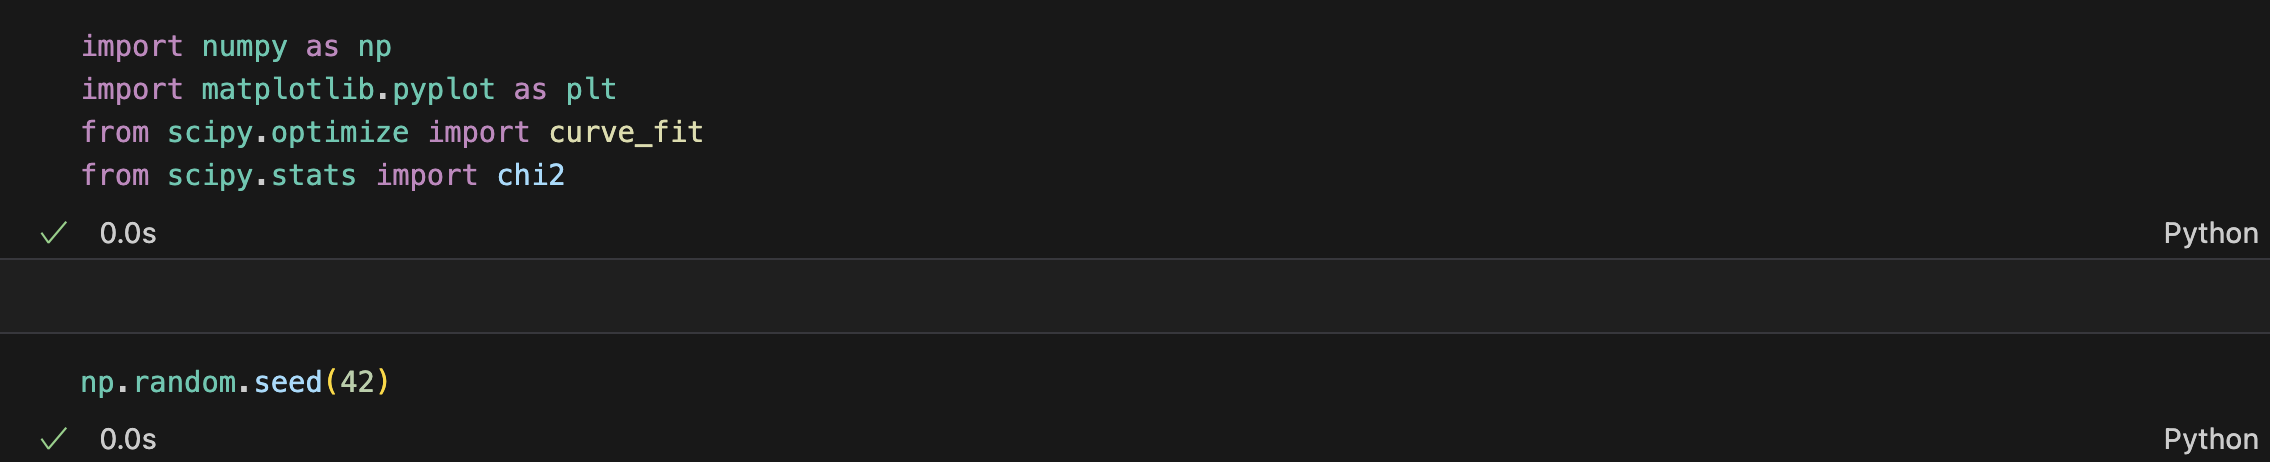
\includegraphics[width=1\linewidth]{figures/code/practice_2/code_2_1.png}
        % \caption{Caption}
        \label{fig:code_2_1}
    \end{figure}
    \begin{figure}[h]
        \centering
        
\includegraphics[width=1\linewidth]{figures/code/practice_2/code_2_2.png}
        % \caption{Caption}
        \label{fig:code_2_2}
    \end{figure}
    % \begin{figure}[h]
    %     \centering
    %     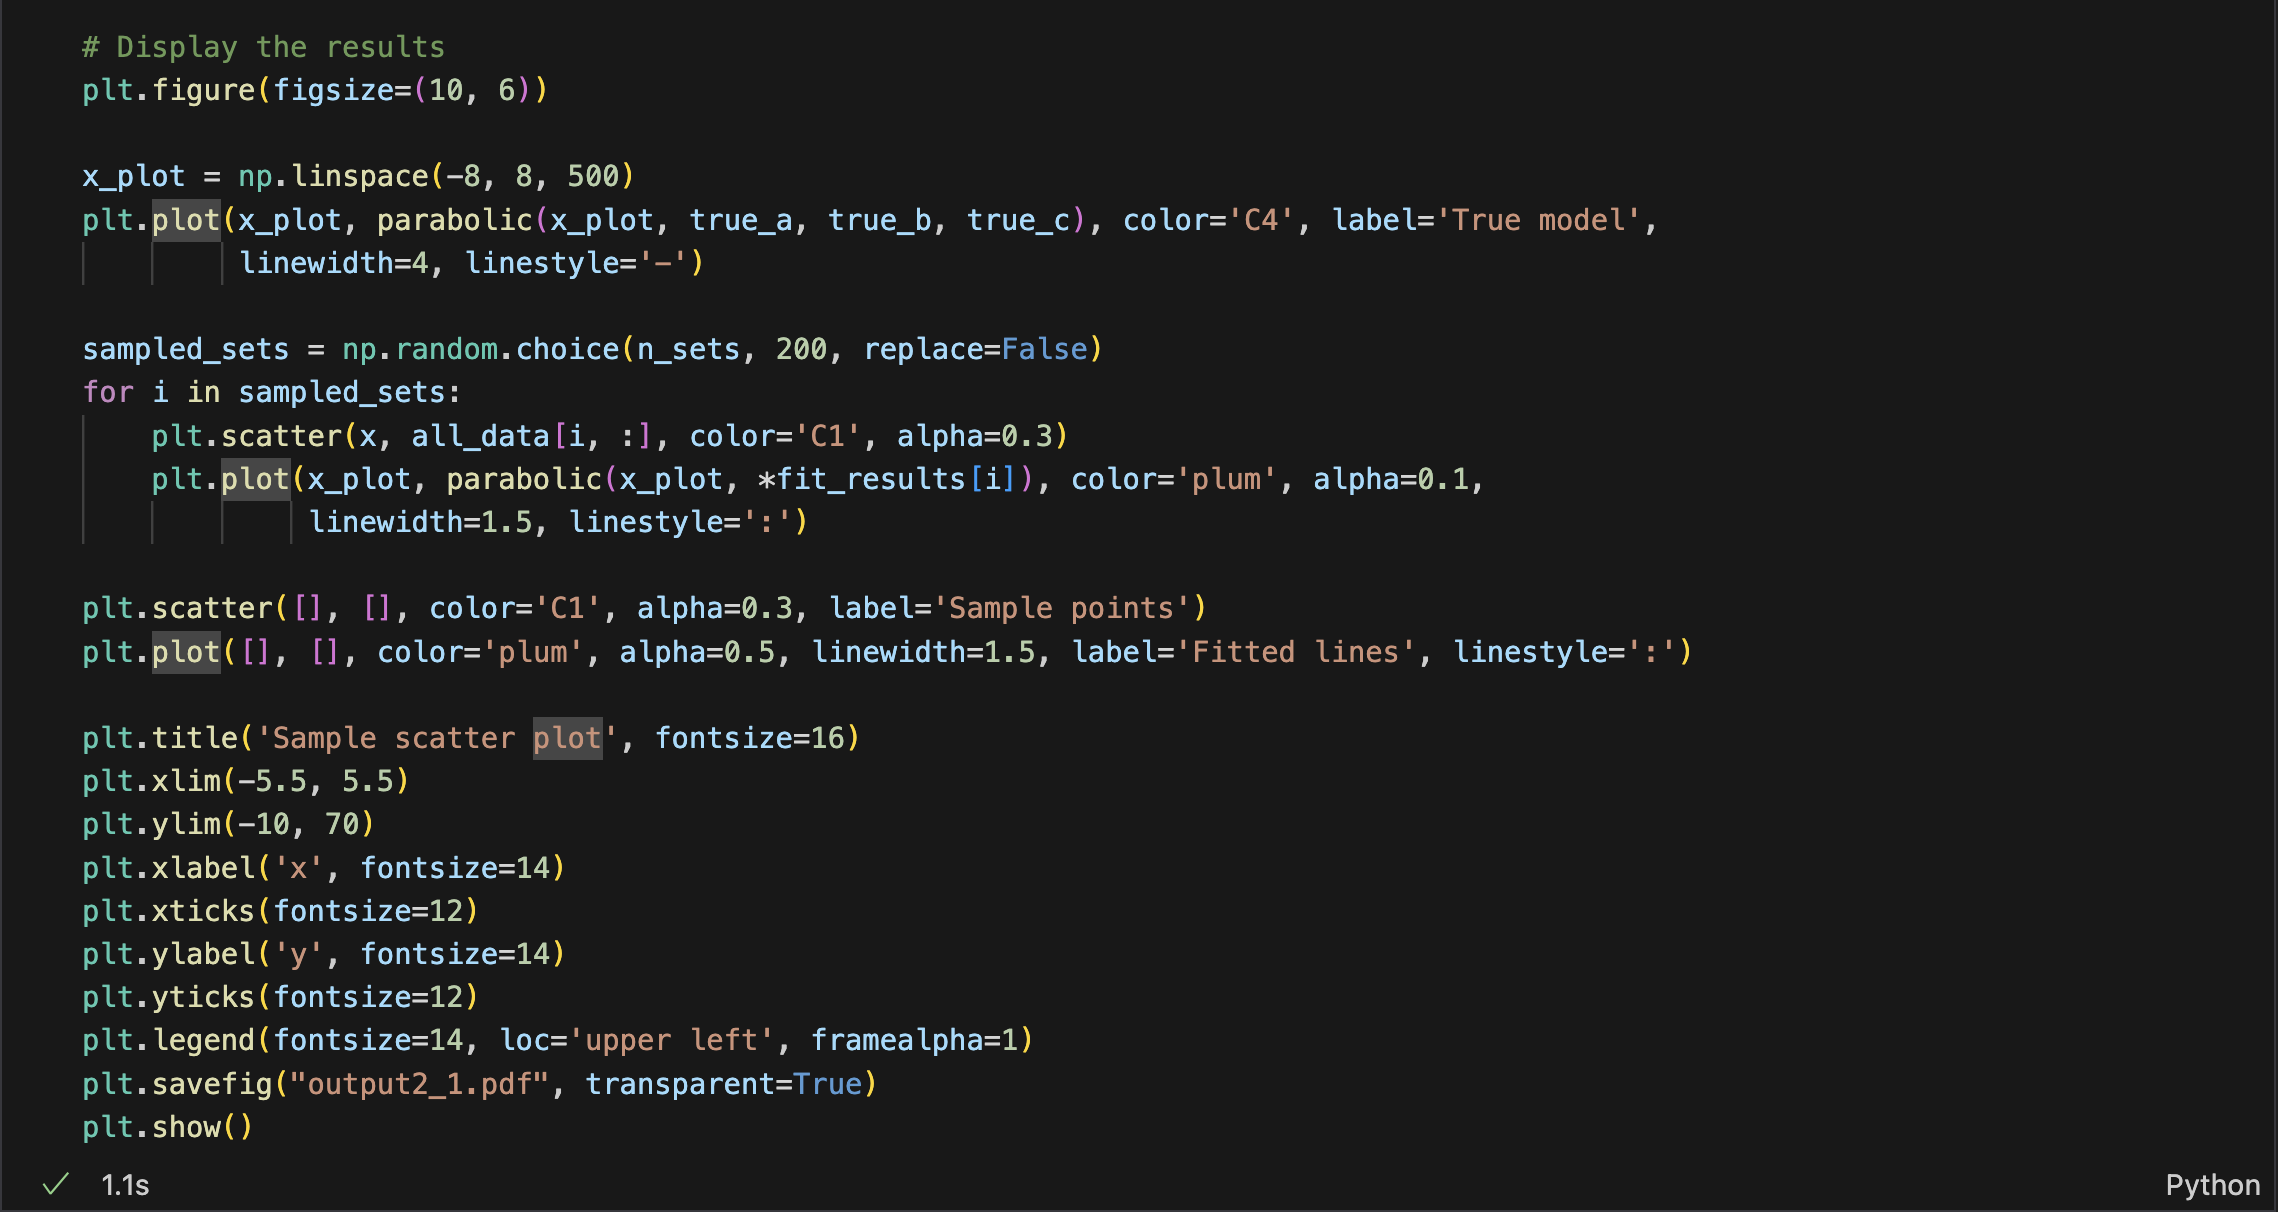
\includegraphics[width=1\linewidth]{figures/code/practice_2/code_2_4.png}
    %     % \caption{Caption}
    %     \label{fig:code_2_4}
    % \end{figure}
    % \clearpage
    \item Plot a histogram of the $\chi^2$ values obtained from fitting each dataset.
    % \begin{figure}[h]
    %     \centering
    %     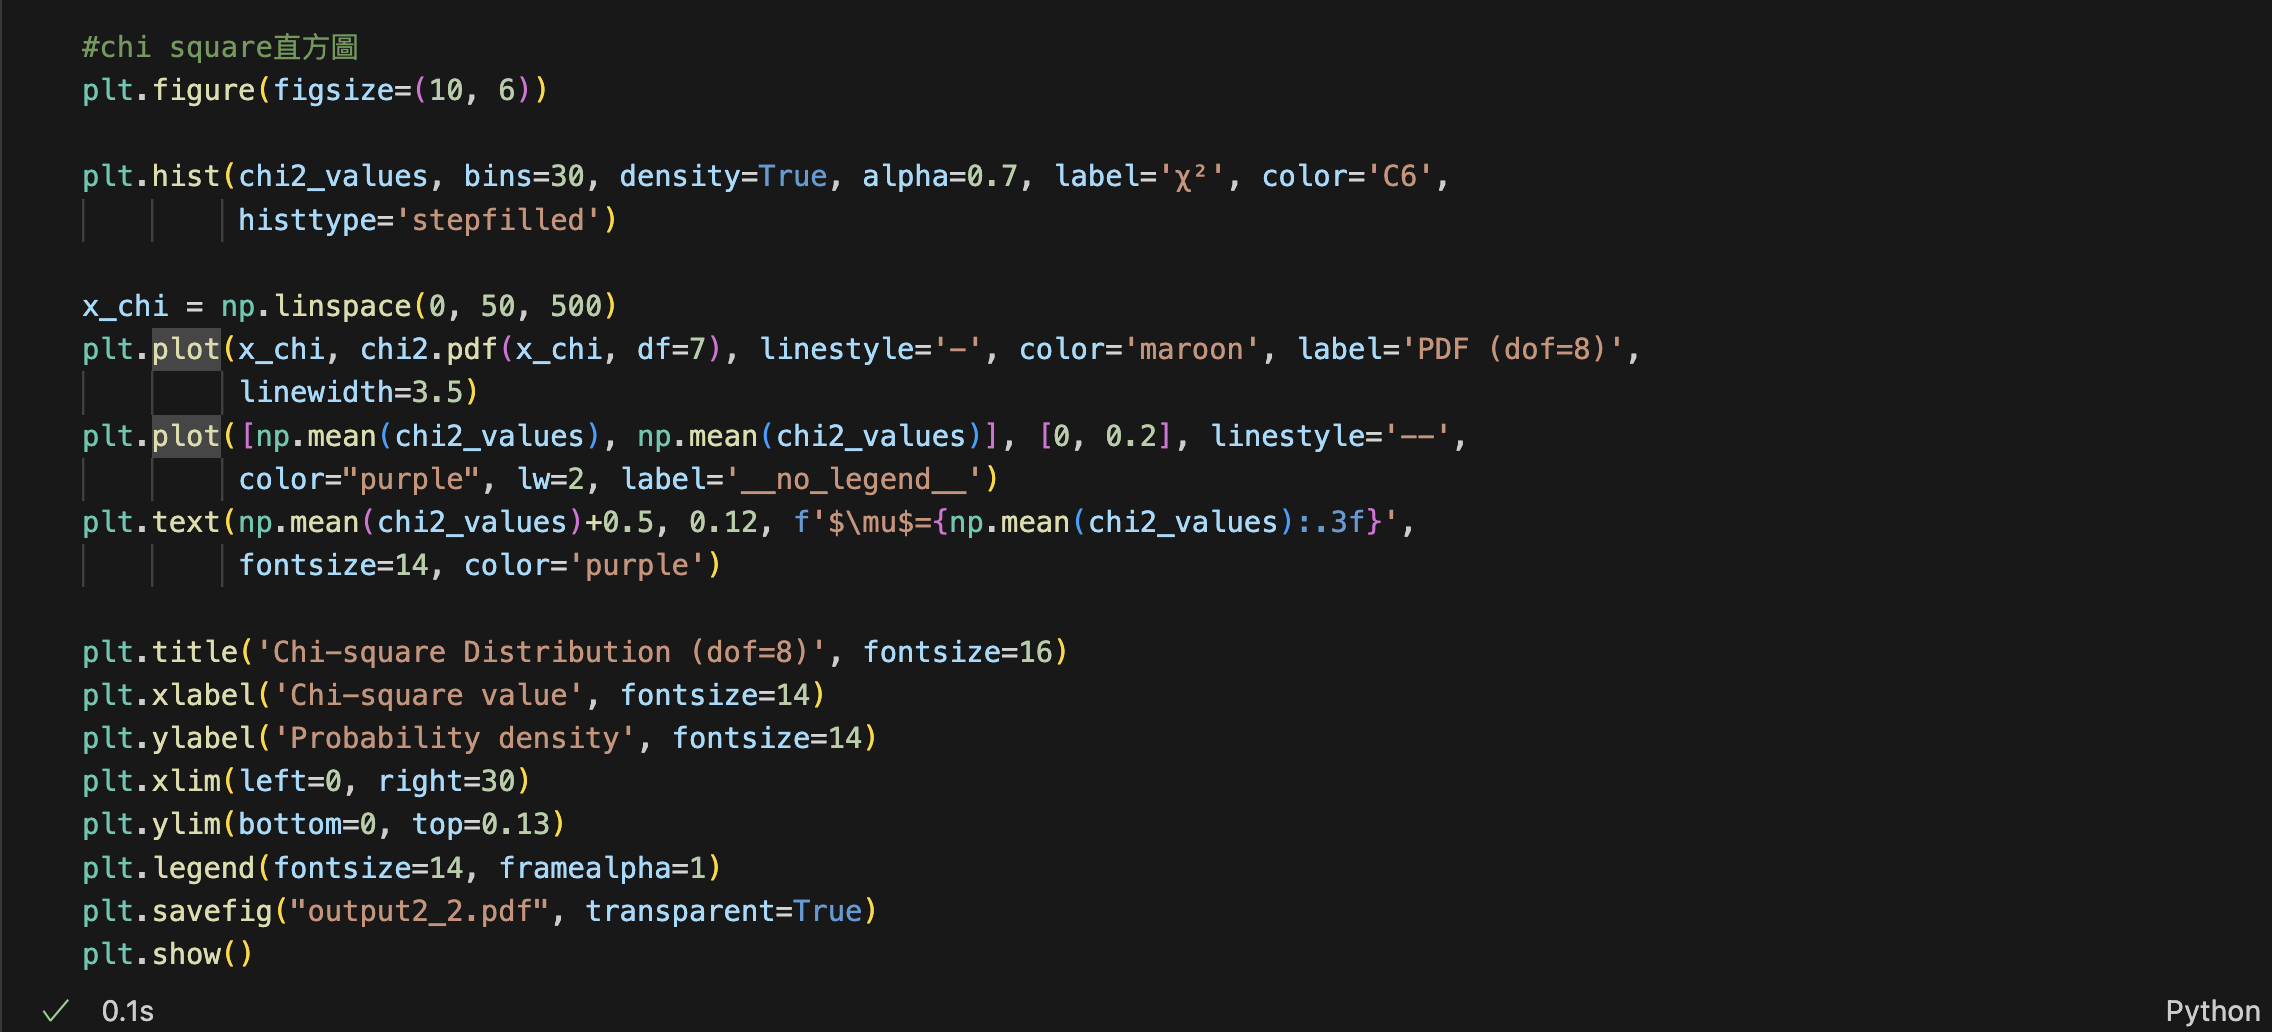
\includegraphics[width=1\linewidth]{figures/code/practice_2/code_2_5.png}
    %     % \caption{Caption}
    %     \label{fig:code_2_5}
    % \end{figure}
    % \clearpage
    \item Mark the \textbf{p-value} get from the fitting result of \texttt{mean(y)}.
    \item You might get a $\chi^2$ of the \texttt{mean(y)} fitting result close to zero and a \textbf{p-value} close to 1.
    % \begin{figure}[h]
    %     \centering
    %     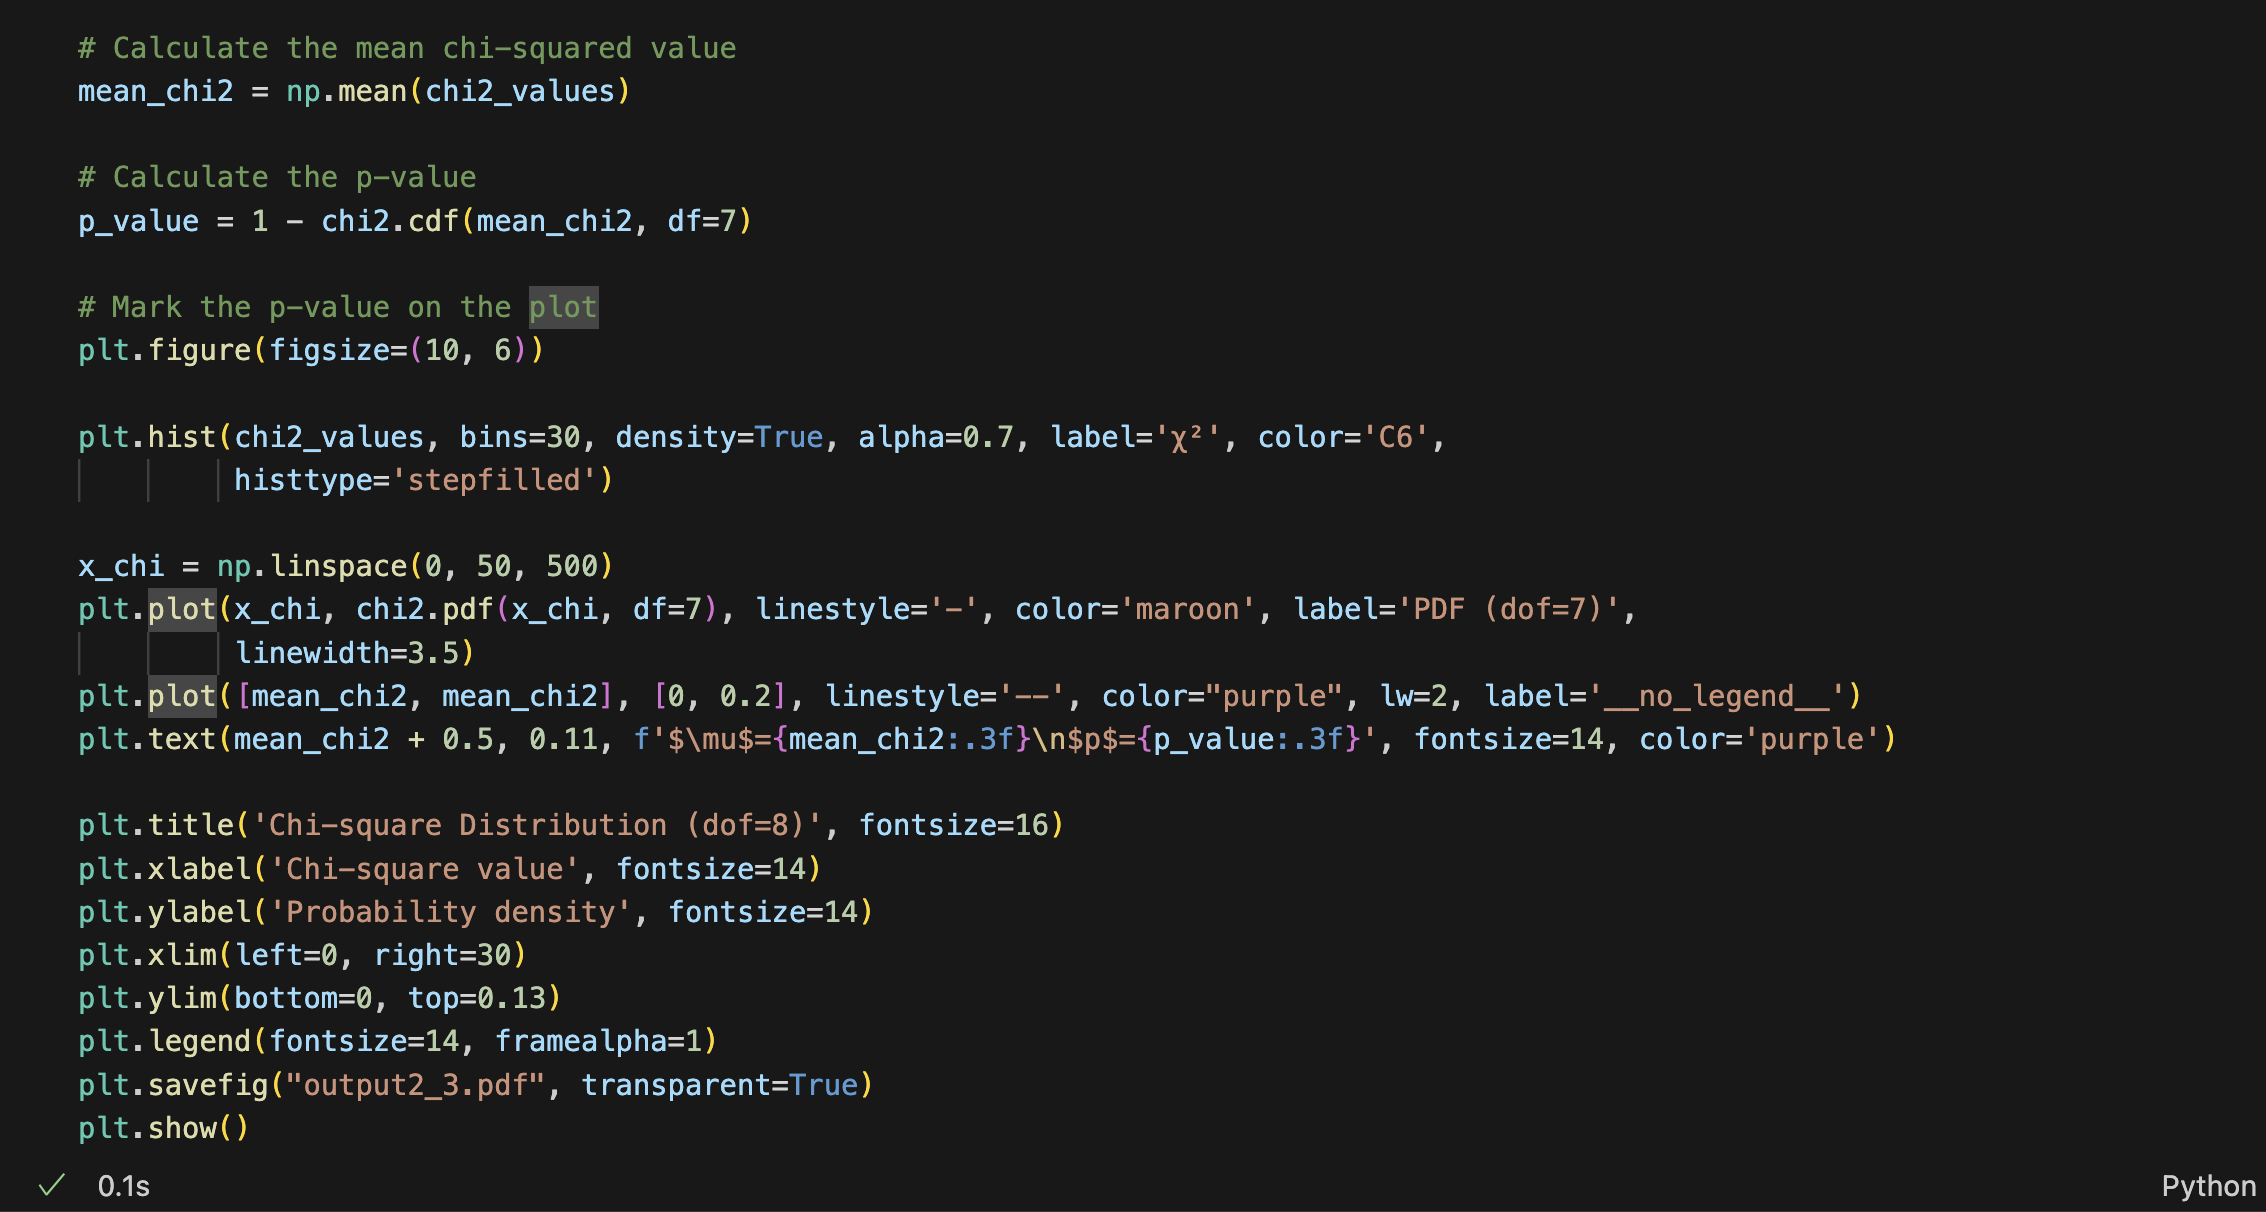
\includegraphics[width=1\linewidth]{figures/code/practice_2/code_2_6.png}
    %     % \caption{Caption}
    %     \label{fig:code_2_6}
    % \end{figure}
    % \clearpage
    \item Also mark \textcolor{blue}{5\% significance level}, and \textcolor{blue}{95\% significance level} on the histogram.
    \begin{figure}[h]
        \centering
        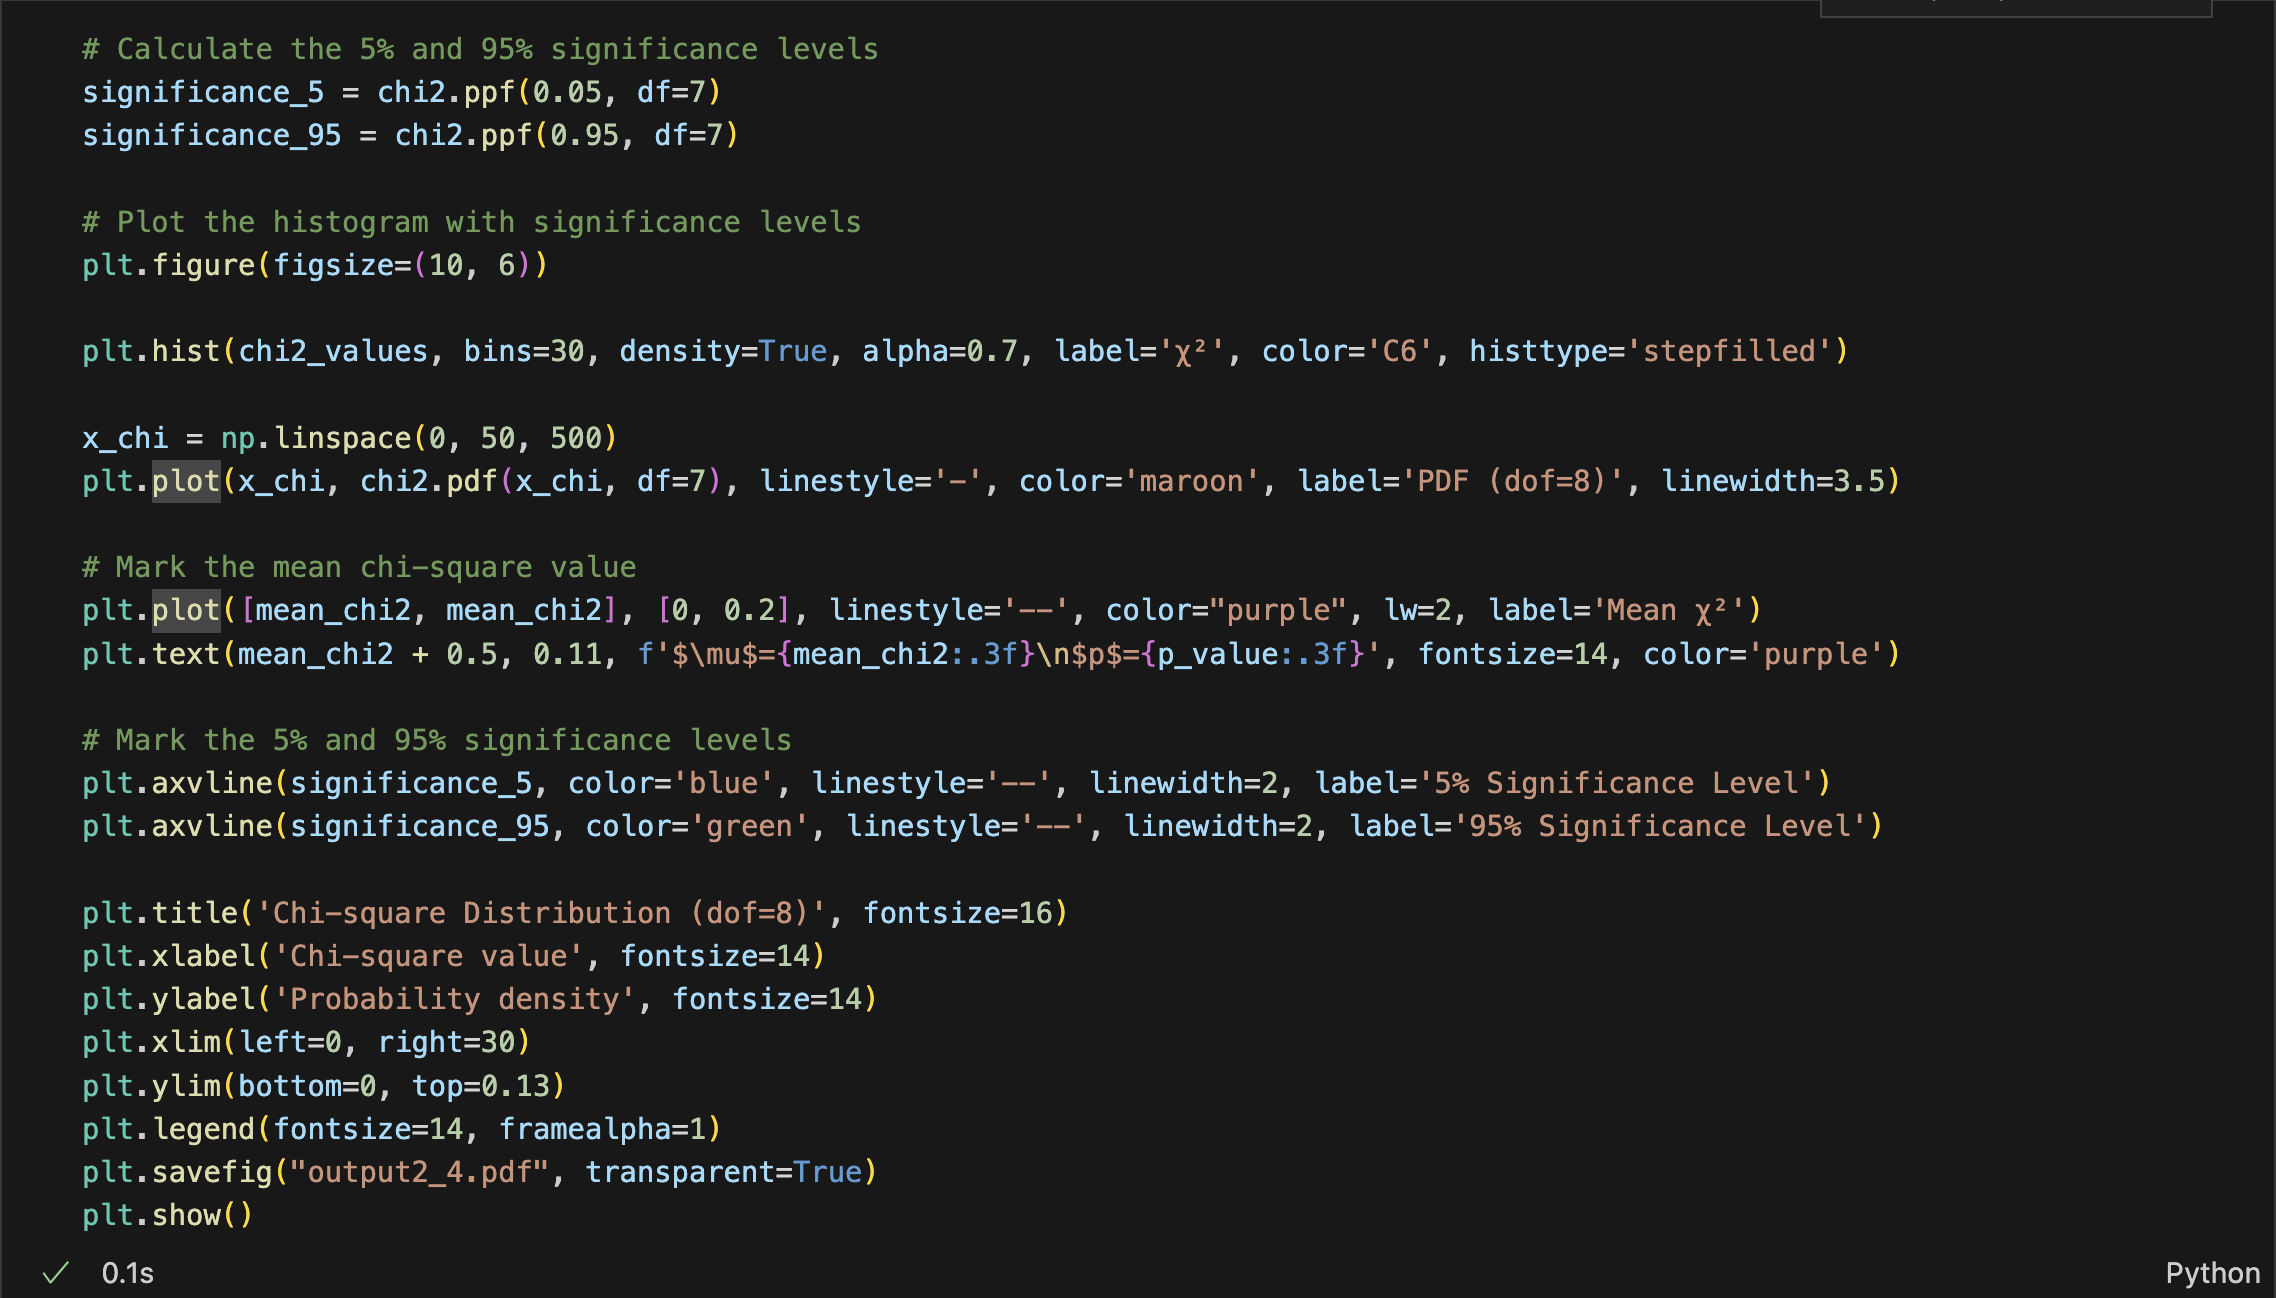
\includegraphics[width=1\linewidth]{figures/code/practice_2/code_2_7.png}
        % \caption{Caption}
        \label{fig:code_2_7}
    \end{figure}
\end{enumerate}


\clearpage
\section{實驗數據與分析}
\subsection{Practice 1}\label{subsec:result_1}
\hfill

\begin{figure}[h]
    \centering
    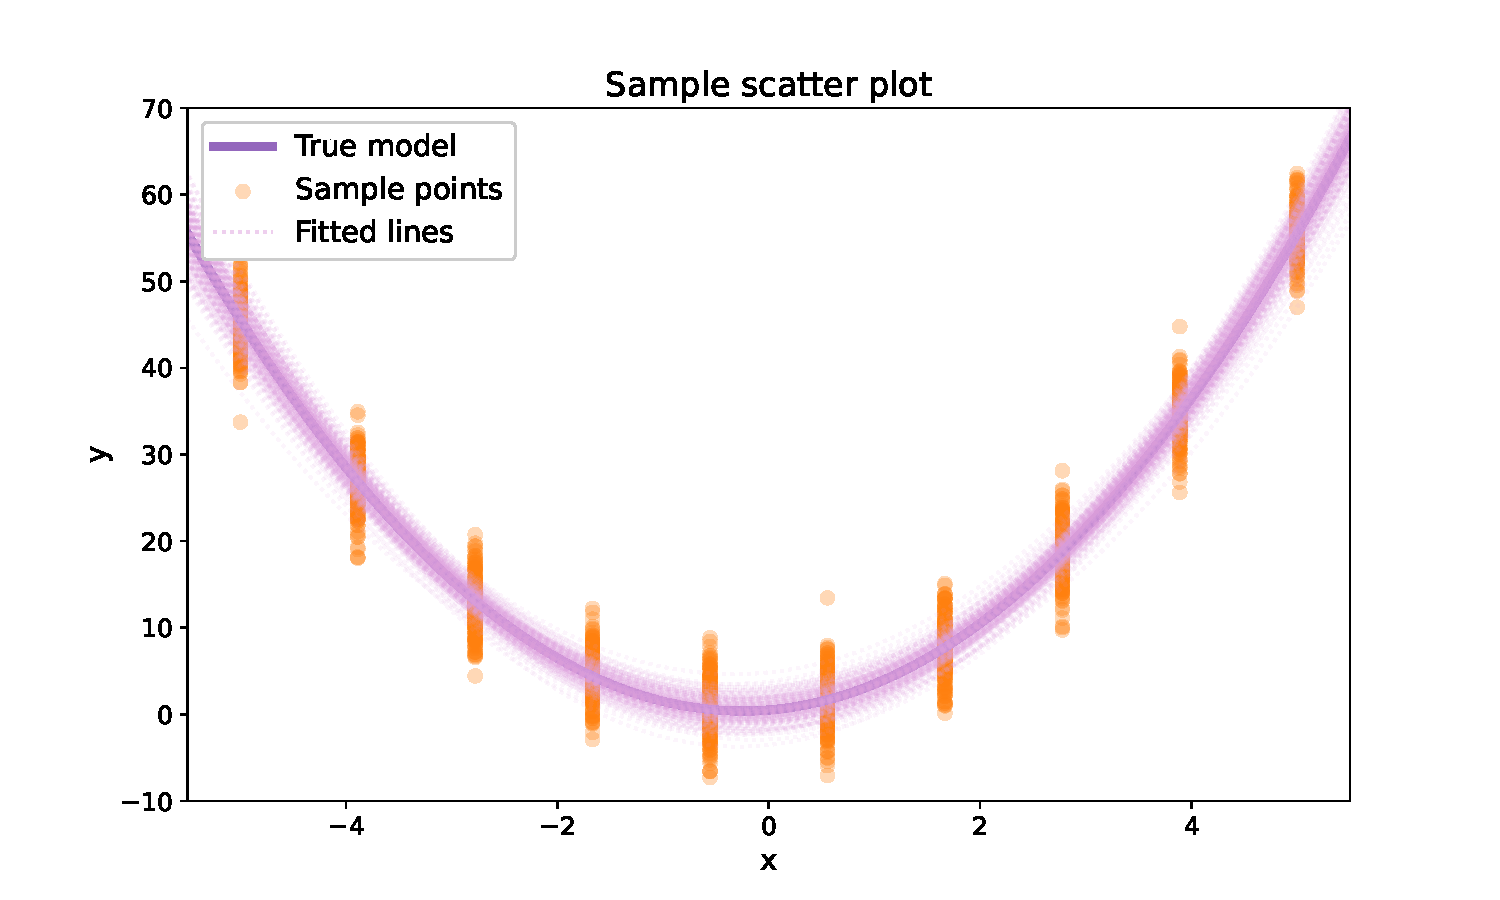
\includegraphics[width=1\linewidth]{figures/output/practice_1/output1_1.pdf}
    \caption{Scatter plot of synthetic data and their fitted parabolas.}
    \label{fig:output1_1}
\end{figure}

Different from the practices of the previous weeks using a linear function to produce experimental data, we tried a different function, i.e., parabola $y=ax^2+bx+c$, to generate our data points to learn and manipulate different scenarios. Fig. \ref{fig:output1_1} shows not only how the synthetic data are scattered, but also how the data are fitted. The chi-square distribution is plotted in Fig. \ref{fig:output2_3} and the mean $\chi^2$ is marked.

To calculate the p-value of the corresponding chi-square without using \texttt{scipy.stats} functions, we referred to the basic definition:
\begin{equation}
    p = P(\chi^2\geq\chi^2_{obs}) = 1 - \text{CDF}_{\chi^2}(\chi^2_{obs}, k)= 1-\frac{\gamma(k/2, x/2)}{\Gamma(k/2)}
\end{equation}
where the $\gamma$ is the lower incomplete gamma function and $\Gamma$ is the gamma function. With this formula, we chose to calculate the p-value of the mean $\chi^2$, which is also labeled in the Fig. \ref{fig:output2_3}.

Moreover, the cumulative distribution function (CDF) of the experimental chi-square and the theoretical distribution are demonstrated in Fig. \ref{fig:output1_4}. As we can see, the empirical CDF (blue solid line) and the theoretical CDF (red dashed line) ideally overlap.

\begin{figure}[h]
    \centering
    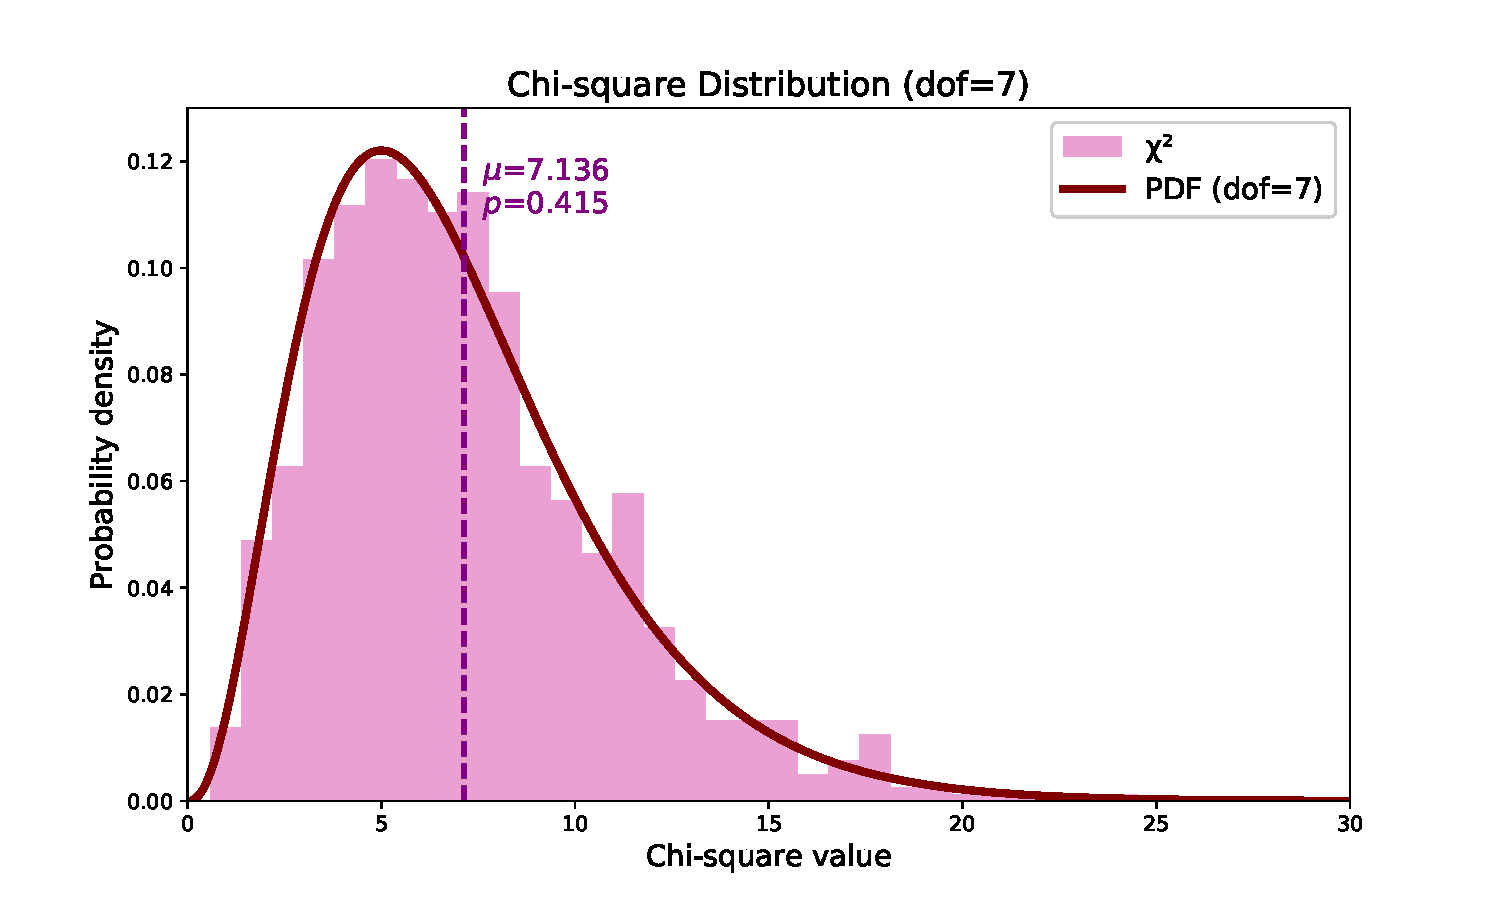
\includegraphics[width=1\linewidth]{figures/output/practice_2/output2_3.pdf}
    \caption{Histogram of the chi-square distribution. The dashed line and text mark the mean $\chi^2$ and its p-value.}
    \label{fig:output2_3}
\end{figure}
\begin{figure}[h]
    \centering
    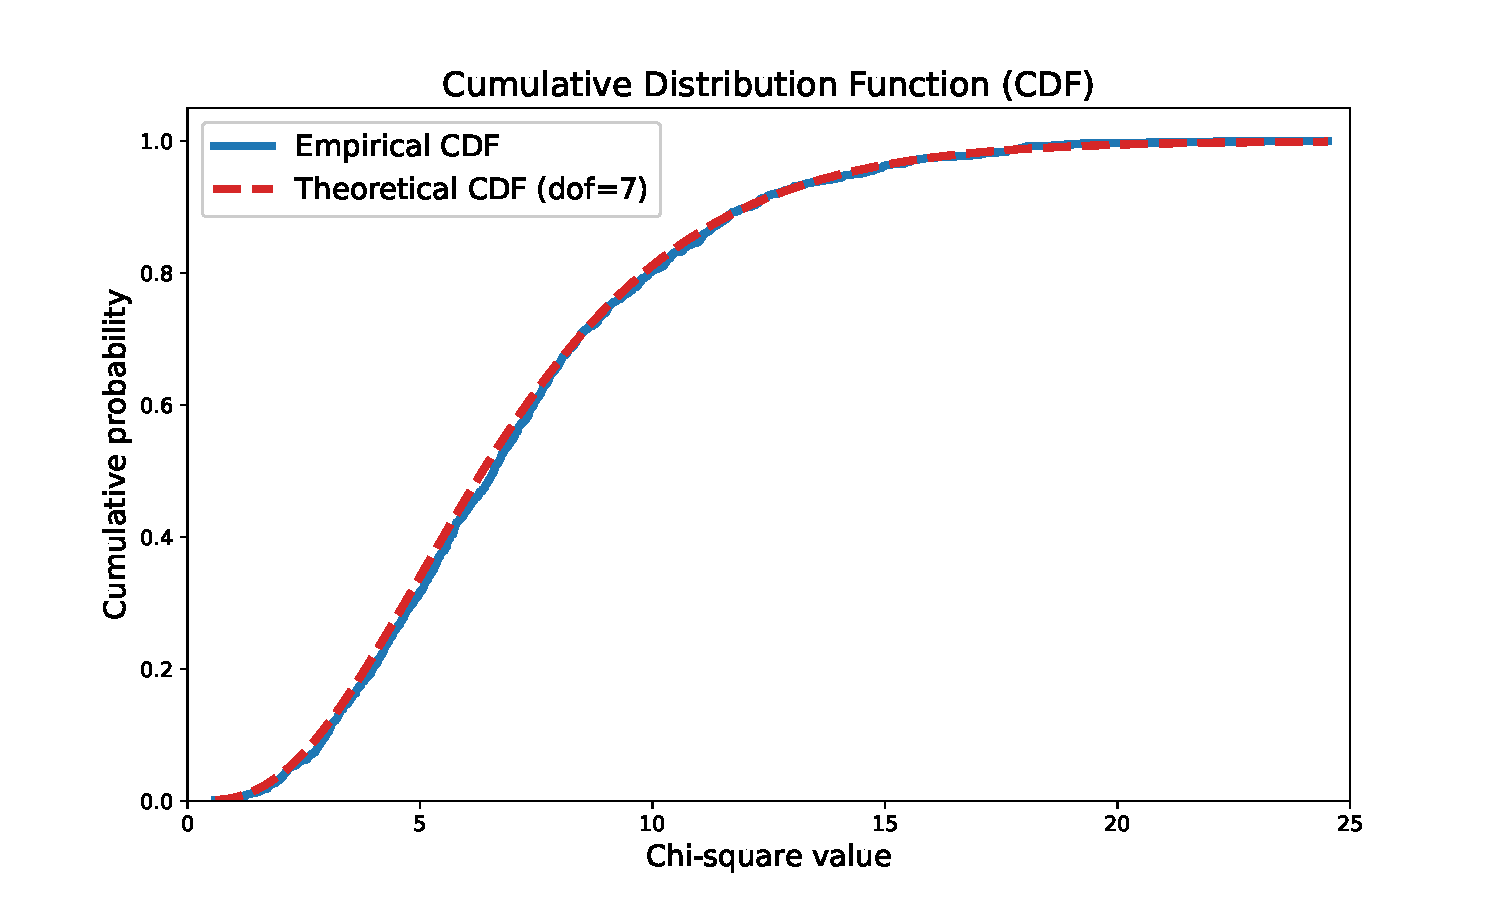
\includegraphics[width=1\linewidth]{figures/output/practice_1/output1_4.pdf}
    \caption{CDFs of the empirical theoretical values}
    \label{fig:output1_4}
\end{figure}

\clearpage
\subsection{Practice 2}
\hfill

% \begin{figure}[h]
%     \centering
%     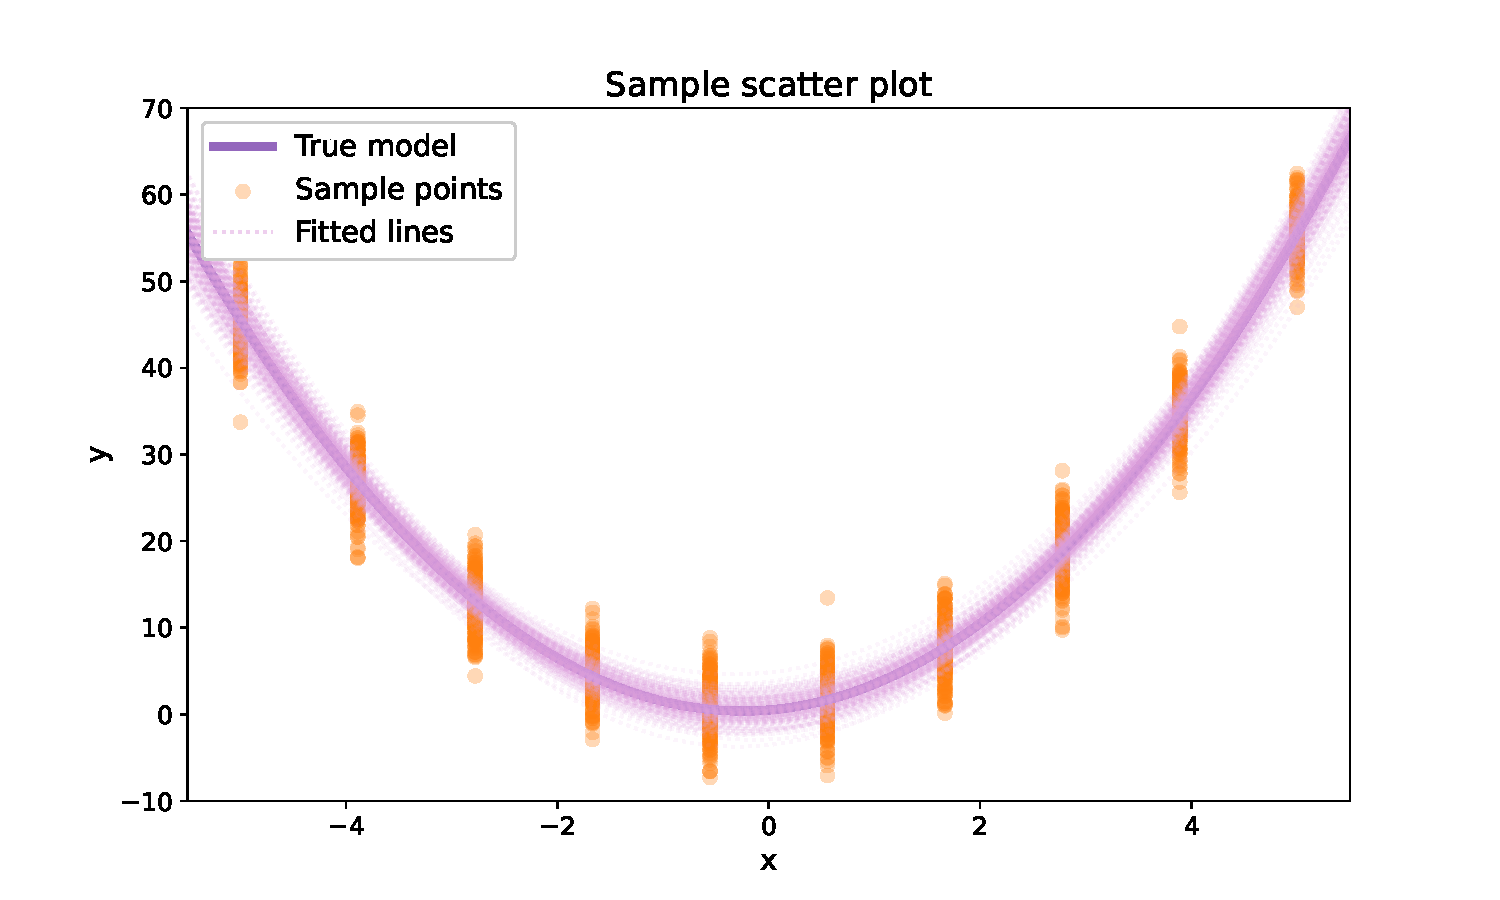
\includegraphics[width=0.8\linewidth]{figures/output/practice_2/output2_1.pdf}
%     \caption{Caption}
%     \label{fig:output2_1}
% \end{figure}

% \begin{figure}[h]
%     \centering
%     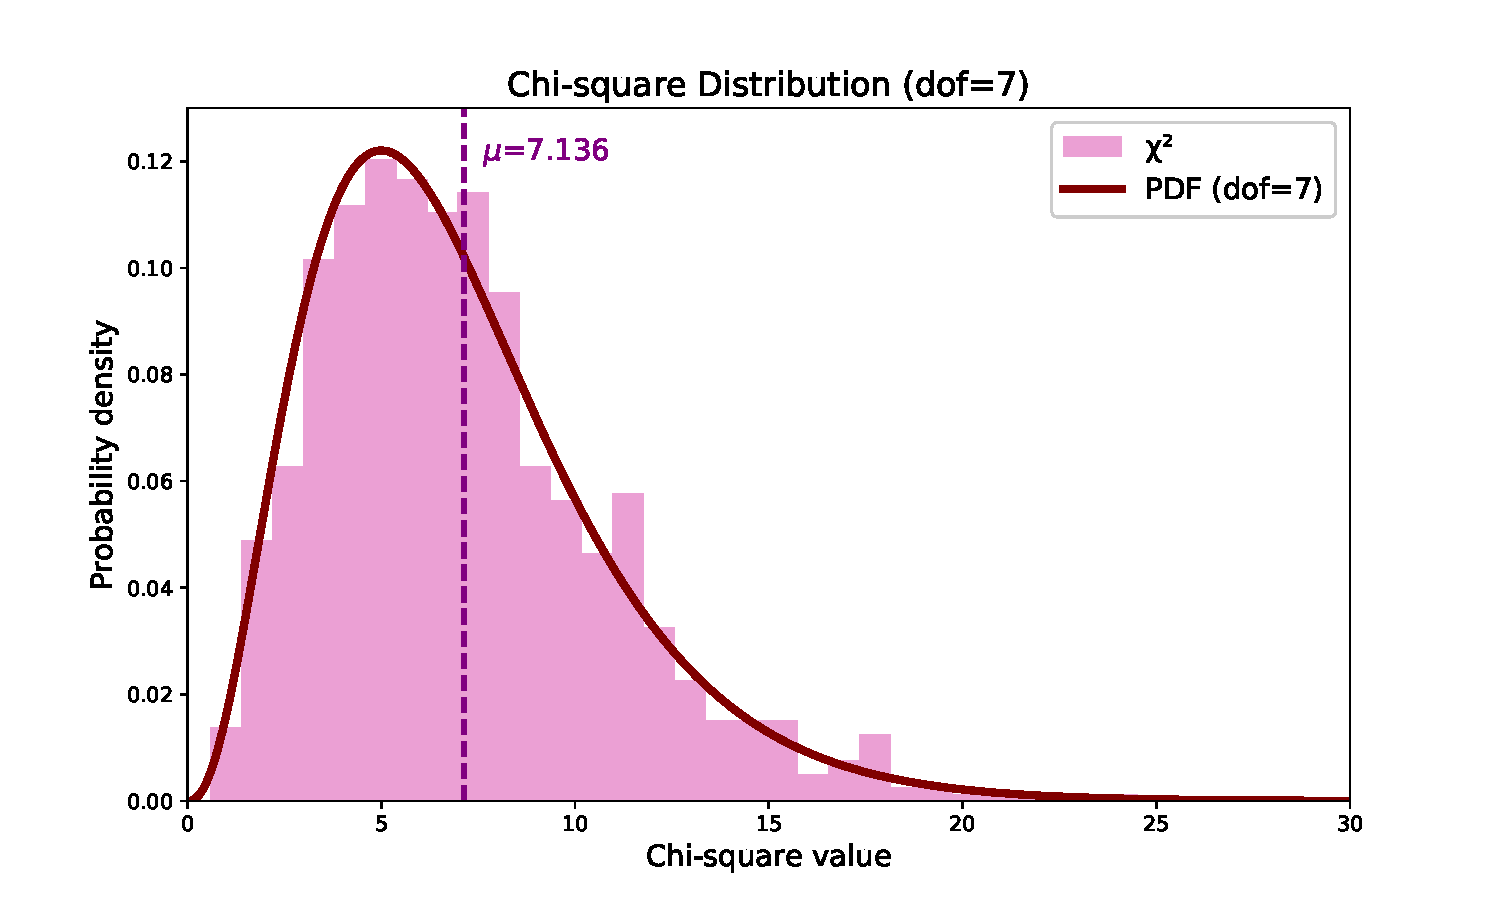
\includegraphics[width=0.8\linewidth]{figures/output/practice_2/output2_2.pdf}
%     \caption{Caption}
%     \label{fig:output2_2}
% \end{figure}

% \begin{figure}[h]
%     \centering
%     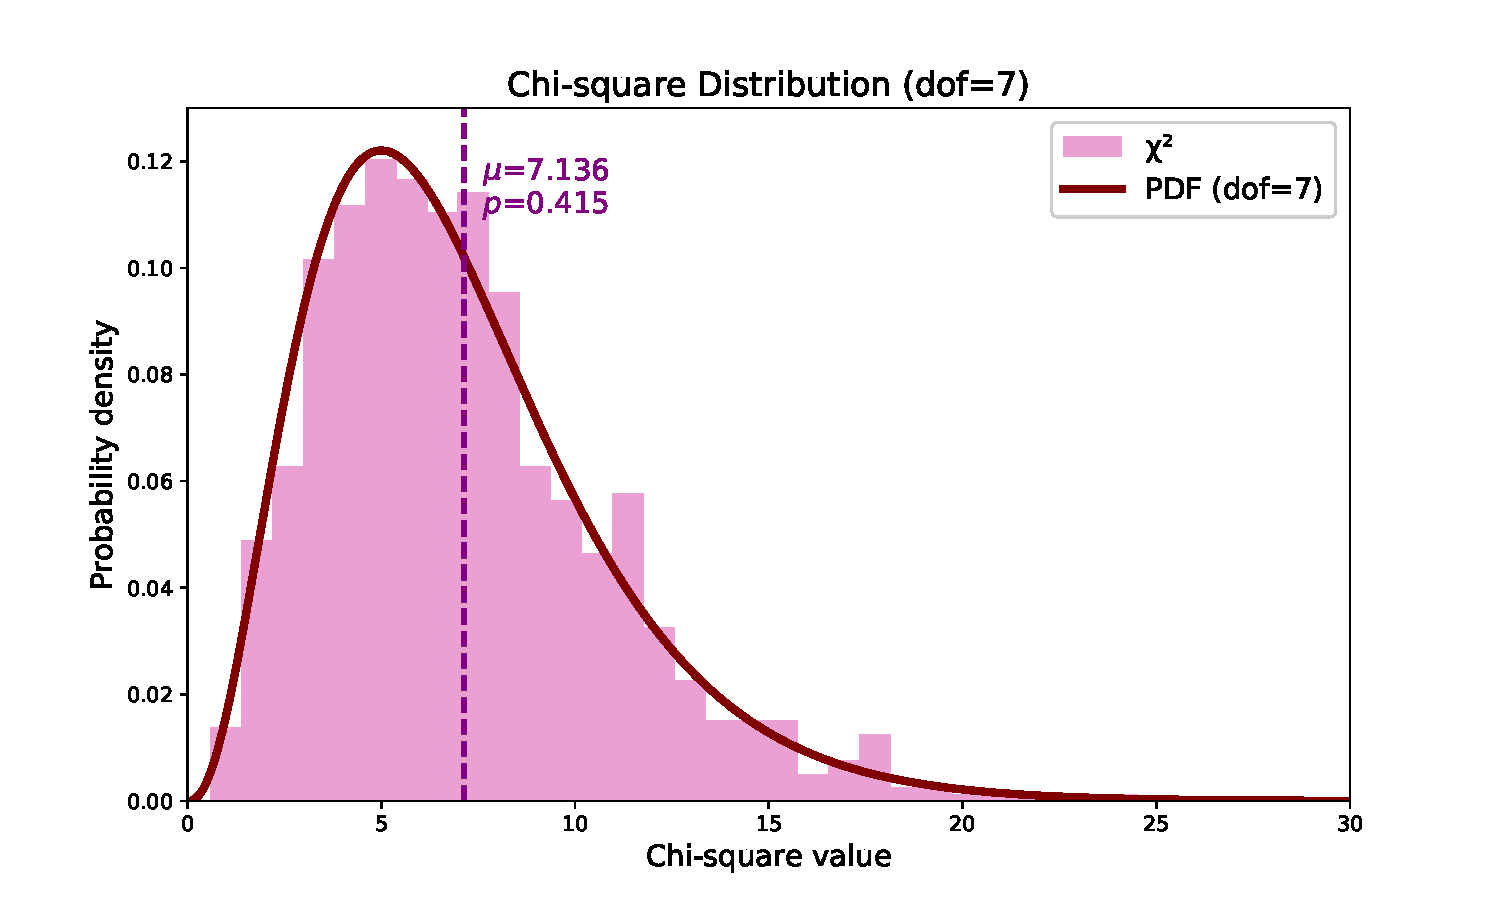
\includegraphics[width=0.8\linewidth]{figures/output/practice_2/output2_3.pdf}
%     \caption{Caption}
%     \label{fig:output2_3}
% \end{figure}
\begin{figure}[h]
    \centering
    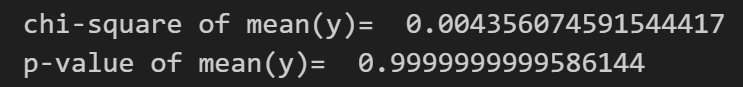
\includegraphics[width=0.8\linewidth]{figures/output/practice_2/output2_3.png}
    \caption{The chi-square of \texttt{mean(y)} and its p-value}
    \label{fig:chisq_p}
\end{figure}

The chi-square of the \texttt{mean(y)}, derived from the fitted line, is 0.004376. Accordingly, the p-value of the chi-square value is extremely close to 1 (the actual values are in the Fig. \ref{fig:chisq_p}). These indeed match our expectation that 'You might get a $\chi^2$ of the \texttt{mean(y)} fitting result close to zero and a \textbf{p-value} close to 1.'

\begin{figure}[h]
    \centering
    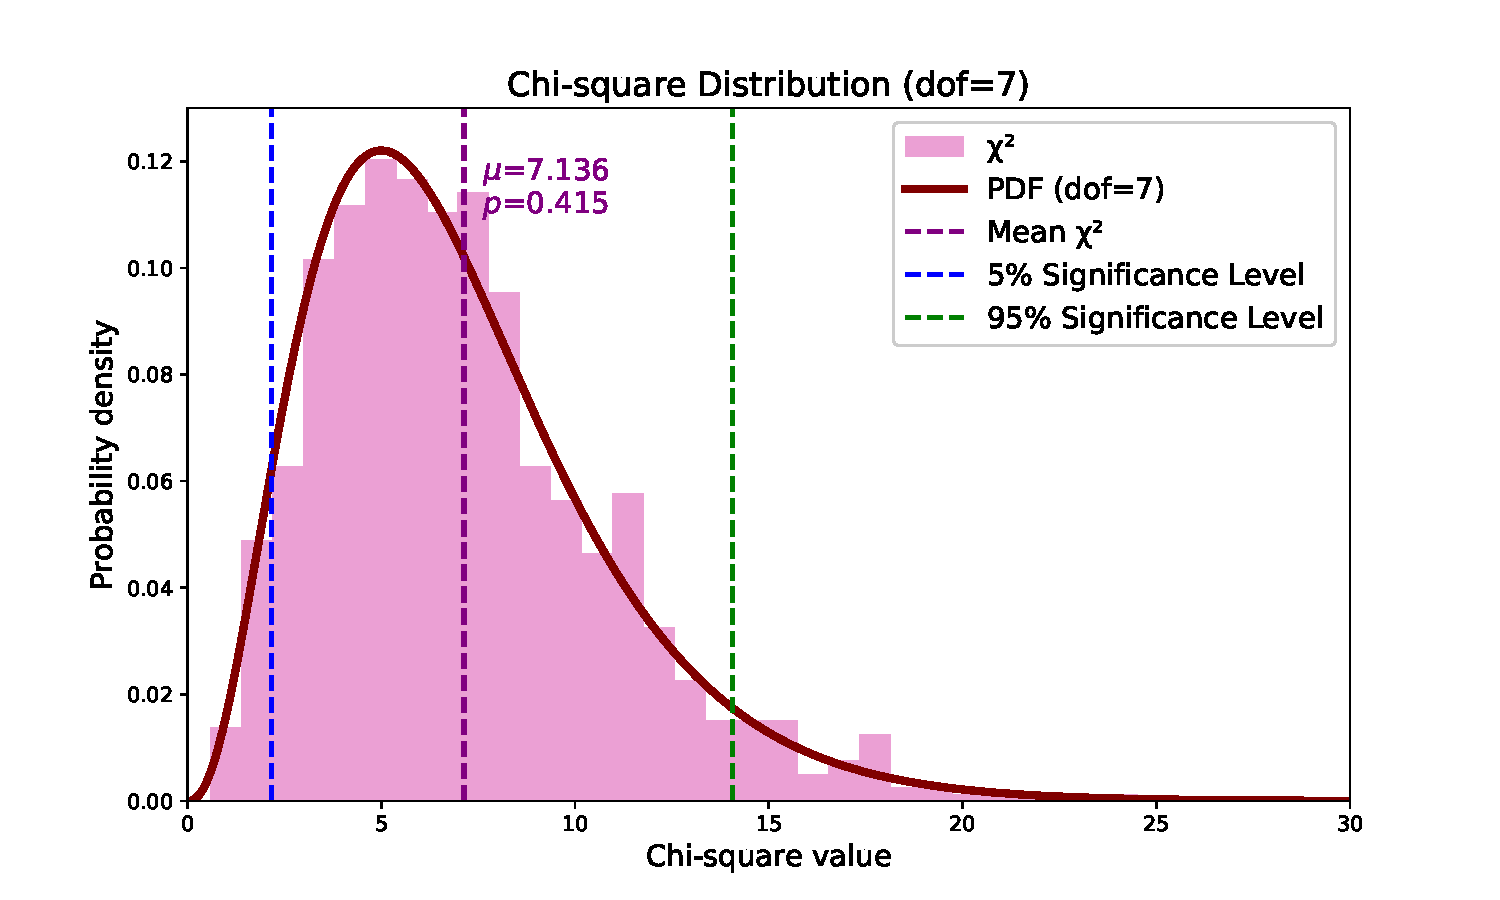
\includegraphics[width=1\linewidth]{figures/output/practice_2/output2_4.pdf}
    \caption{Similar plot as Fig. \ref{fig:output2_3} and the the significant levels of 5\% and 95\% are labeled.}
    \label{fig:output2_4}
\end{figure}


Fig. \ref{fig:output2_4} plots similar characteristics, including the experimental chi-square distribution, the probability density function (PDF) with 7 degrees of freedom, the mean $\chi^2$, and its p-value. Also, with \texttt{scipy.stats. chi2. ppf} to calculate the significance level, 5\% and 95\% are marked with blue and green dashed lines, respectively. The area between 5\% and 95\%  significance level is roughly the same as the Fig. \ref{fig:sig_level}.

Further discussion and analysis of chi-square, p-value, and significance level are in the following section.

\clearpage
\section{問題討論}
\subsection{Practice 1}\label{subsec:discuss_1}

\subsubsection{Will the fitted parameters be closer to the initial parameters you set to generate the data points with larger \textbf{p-value}? You should trust your results rather than rely on preconceived bias.}
\hfill

我們選出各選出$p<0.05$、$0.4<p<0.6$、$p>0.9$的其中一組資料,並繪出對應之最佳擬合參數所建立的模型與true model比較。

\begin{figure}[h]
    \centering
    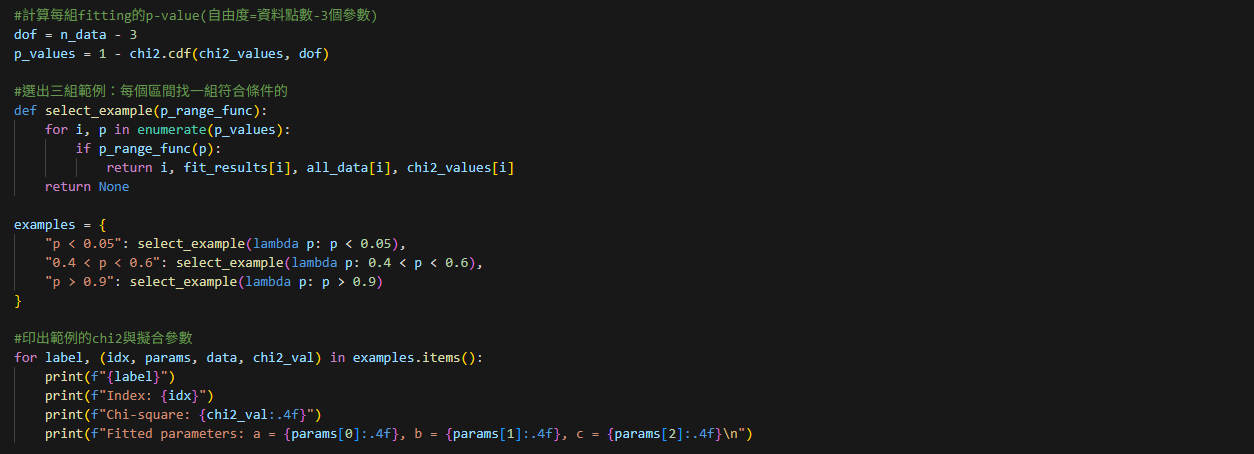
\includegraphics[width=1\linewidth]{figures/RF/practice_1_QA_1.png}    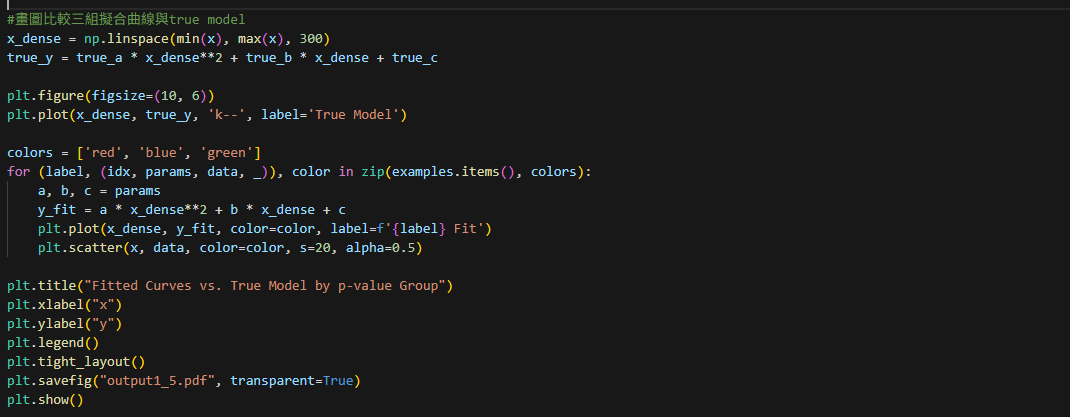
\includegraphics[width=1\linewidth]{figures/RF/practice_1_QA_2.png}
    %\caption{Enter Caption}
    \label{fig:code_p1QA}
\end{figure}

\clearpage

\begin{figure}[h]
    \centering
    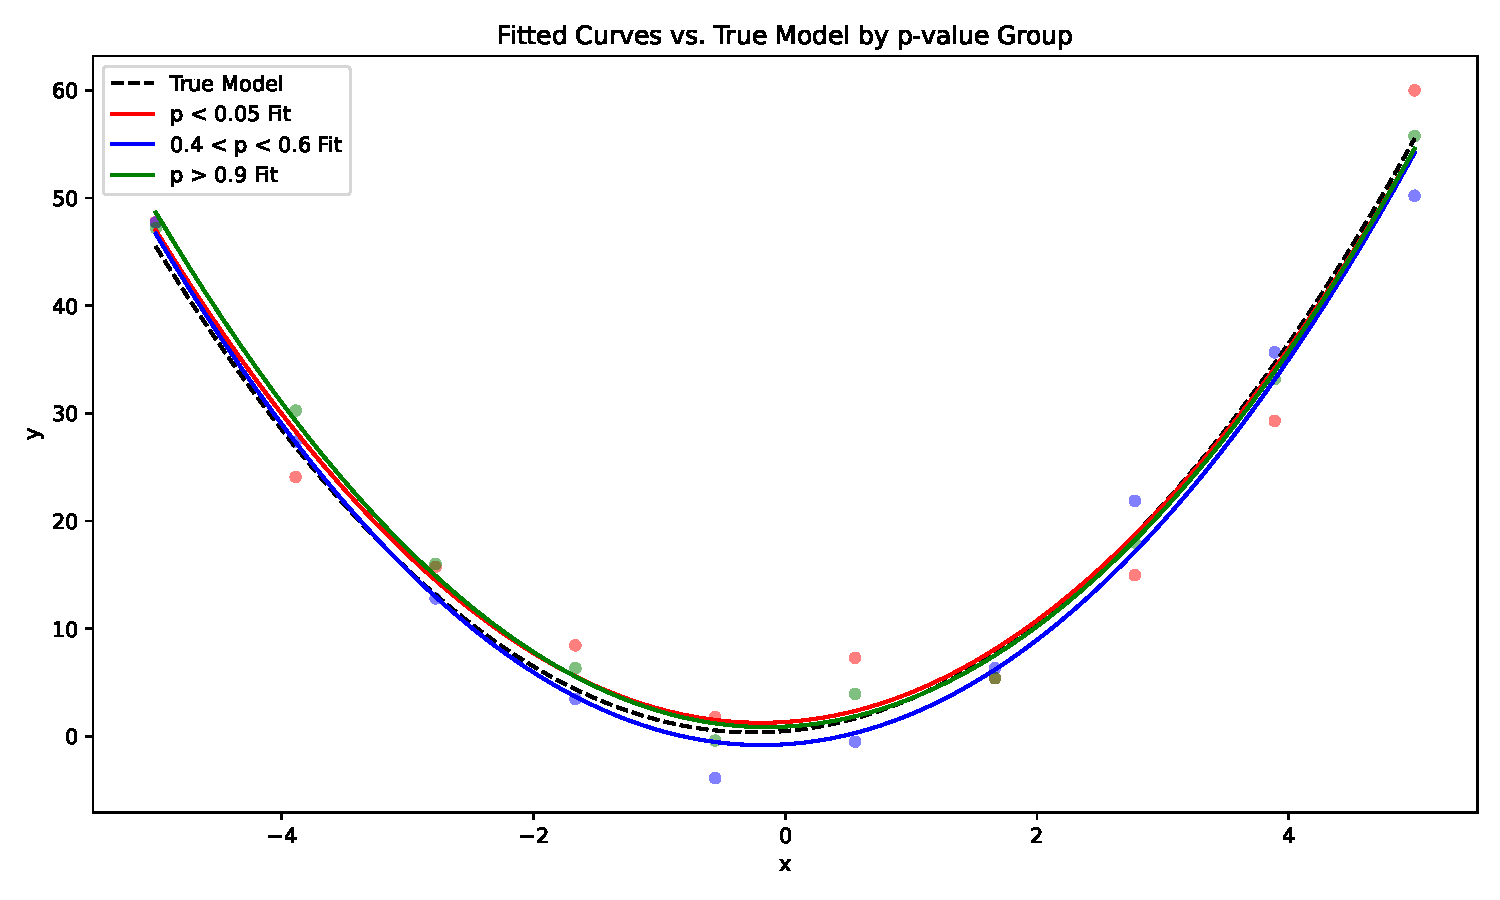
\includegraphics[width=1\linewidth]{figures/RF/output1_5.pdf}
    \caption{選三種不同情況的p-value對應之數據,與true model比較}
    \label{fig:enter-label}
\end{figure}

每一組詳細資料:
\begin{itemize}
    \item $p < 0.05$
    \begin{itemize}
        \item Index: 60
        \item Chi-square: $14.1291$
        \item Fitted parameters: $a = 1.9778$, $b = 0.7572$, $c = 1.3412$
    \end{itemize}
    \item $0.4 < p < 0.6$
    \begin{itemize}
        \item Index: 4
        \item Chi-square: $6.4121$
        \item Fitted parameters: $a = 2.0462$, $b = 0.7519$, $c = -0.7291$
    \end{itemize}
    \item $p > 0.9$
    \begin{itemize}
        \item Index: 21
        \item Chi-square: $2.0211$
        \item Fitted parameters: $a = 2.0284$, $b = 0.5925$, $c = 0.9131$
    \end{itemize}
\end{itemize}

\clearpage

\begin{table}[h]
    \centering
    \begin{tabular}{|c|c|c|c|}
        \hline
        原始數據&$p<0.05$&$0.4<p<0.6$&$p>0.9$\\
        \hline
        $a=2.0$&1.11\%&24.3\%&160\%\\
        \hline
        $b=1.0$&2.31\%&24.8\%&246\%\\
        \hline
        $c=0.5$&1.42\%&40.8\%&82.6\%\\
        \hline
    \end{tabular}
    \caption{每組擬合參數與原始設定的誤差}
    \label{tab:2}
\end{table}

雖然統計的理論上,較高的$p-value$通常表示擬合結果會較為精準,所以會預期擬合出來的參數會更接近原始設定的數值。然而,Tab.\ref{tab:2}卻反映了不一樣的結果。
\begin{itemize}
    \item 在$p>0.9$那組數據中,理應預期他的誤差要最小,結果它的誤差卻是最大的,甚至比起其餘二組有非常明顯的差距。
    \item $p<0.05$預期是擬合結果最差的,結果它反而是最接近true model的數據。
\end{itemize}

這說明了$p-value$雖然可以反映出擬合後與資料的吻合程度,但其實不能保證擬合後的參數繪最接近真實情況;當然也可能是因為我們是隨機選擇每一組的數據,或許剛好選到的參數是偏離原始值較多的一組。所以我們不能預設「p-value越大擬合參數就會越準」,還是要根據實際的擬合結果判斷,而且也不能單就依賴p-value作為唯一依據,應該要搭配更多的方式做更全面的統計分析。

\subsection{Practice 2}

\subsubsection{State the goodness of fitting result by comparing the \textbf{p-value} with the significance level.}
\hfill

p-value 以及 significance level的定義在本實驗報告前言部分已詳細介紹。在這次實驗中,我們設定的significance level為 5\% 和 95\% ,這是我們判斷擬合結果好壞的標準。如果擬合的結果對應到的 p-value 數值在 $0.05$ 到 $0.95$ 之間,就代表此數據的 $\chi^2$ 值落在合理的範圍內,擬合結果與理論模型相符,沒有顯著偏差,表示擬合結果良好。如果p-value 小於 0.05 或大於 0.95,則代表這筆擬合結果比較極端,不符合預期的理論數值:$\chi^2$ 過大是欠擬合、$\chi^2$ 過小過擬合。代表這個模型並不適用於此數據擬合。

\subsubsection{If the \textbf{p-value} get from the fit is less than 0.05, what does it mean?}
\hfill

初始假設是此模型適用於此次擬合,但是 p-value 小於 $0.05$ ,代表在虛無假設為真的情況下,產生目前擬合結果的機率非常低,表示擬合結果與理論模型有很大的差異,因此可以認定這是不合理的結果,並且拒絕原本的模型假設,把此次擬合判定為不合理的結果。

\subsubsection{Make a conclusion how to make an accurate statement about the goodness of fitting result.}
\hfill

\begin{enumerate}
    \item 比較p-value 與significance level,若 p-value 落在設定的significance level 的區間內,就表示該擬合結果統計上合理。
    \item 比較$\chi^2$ 值與自由度,若$\chi^2$ 值與自由度接近,即代表擬合品質佳。
    \item 利用數據繪製成圖表,可確認趨勢是否符合預期或擬合曲線是否足夠貼合資料點與真實模型。
    \item 繪製殘差圖或者與理論CDF做比較,確認有無系統性偏差。
\end{enumerate}

%%%%%%%%%%%%%%%%

\section{總結}
\hfill

本次實驗透過兩個練習深入探討了 p-value 在統計檢定中的意涵,並實際操作卡方擬合的過程。從實驗結果得知,p-value 能有效判斷模型擬合結果是否偏離理論預期,當其落在設定的顯著水準(如 5\% 到 95\%)範圍內,即可視為擬合合理。此外,我們也觀察到 p-value 的大小不一定與模型參數的準確性成正比,說明在評估擬合品質時,應搭配其他統計工具與視覺化圖表進行綜合判斷,例如殘差分析與 CDF 比對。最後,本實驗不僅加深了我們對統計理論的理解,也提升了使用 Python 進行資料處理與圖像化呈現的能力,為後續更進階的實驗與研究奠定良好基礎。


\section{分工}
\begin{itemize}
    \item 洪瑜: 實驗分析、問題討論
    \item 黃巧涵: 實驗分析、問題討論
    \item 洪懌平: 實驗分析
\end{itemize}


% \clearpage
\section{Appendix}

\subsection{Source code}

\begin{itemize}
    \item \url{https://github.com/hyp0515/exp_phy_ii/tree/main/may13}
\end{itemize}

\subsection{References}
\begin{itemize}
    \item \url{https://www.yongxi-stat.com/hypothesis-stat/}
    \item \url{https://rpubs.com/Hsuan_/915898}
    \item \url{https://homepage.ntu.edu.tw/~clhsieh/biostatistic/6/6-7.htm}
    \item \url{https://homepage.ntu.edu.tw/~huilin/2008-1/ch11.pdf}
\end{itemize}
%--------------------------------------------------------------%
\end{CJK}
\end{document}